\documentclass[11pt, oneside]{amsart}

\usepackage[old, colour]{jack}
\def\arraystretch{1}
\title{Group theory}
\author{Jack DeSerrano}
\date{\today}
\usepackage{dynkin-diagrams}

\begin{document}



\tikzset{
        dot/.style = {circle, fill = black,inner sep=0pt,minimum size=4pt, node contents={}},
        every label/.style = {inner sep=1pt, font=\footnotesize}
    }
\maketitle
These notes are based on Richard Borcherds's YouTube series on group theory (at \url{https://www.youtube.com/playlist?list=PL8yHsr3EFj51pjBvvCPipgAT3SYpIiIsJ}.)

\tableofcontents
\newpage

\section{Introduction}
A symmetry is a way of mapping something to itself while preserving that thing's structure, and a \defn{group} is a collection of the symmetries of something. We can consider the Platonic solids, for instance. 

What symmetries does the dodecahedron have? We can rotate it about an axis going through two opposite faces; whenever we rotate it by $1/5$ of a revolution about this axis, it will appear the same, so this rotation is a symmetry. 

We might also rotate it about an axis going through opposing vertices; if we rotate it by $1/3$ of a revolution about this axis, it will appear the same, so this rotation is also a symmetry. Please refer to figure 1 for a rough visual.
\begin{figure}
\centering
\includegraphics[scale=0.4]{images/dodecahedron}
\caption{The rotational symmetries of a dodecahedron.}
\end{figure}

We call the first symmetry a symmetry of \defn{order} $5$, and the second a symmetry of order $3$; this refers to how many times you apply the symmetry to get back to where you started. The dodecahedron also has symmetries of order $2$ corresponding to flipping it about opposite edges and one symmetry of order $1$ corresponding to doing nothing. 

How many symmetries does the dodecahedron have? It turns out that it has $60$ symmetries, corresponding to the $5$ rotations of each face and the $12$ faces.

The cube has $24$ symmetries, the octahedron $24$, the icosahedron $60$, and the tetrahedron $12$. We should notice that the cube and the octahedron and the dodecahedron and the icosahedron have the same number of symmetries. This fact is no coincidence, and we will explore it later.

We call the rotational symmetry group of order $5$ \defn{cyclic} of order $5$, which we will write as $\Z/5\Z$.

We can also form the symmetry group of $n$ identical objects. There are $n!$ of these symmetries, and we call the corresponding group the \defn{symmetric group} on $n$ objects and denote it $\Sg_n$. 

We can also consider the group of symmetries of a vector space over a field. Let's consider $\R^3$ over $\R$. We can let the symmetries here be the maps that preserve addition and multiplication by real numbers, given by all invertible $3\times 3$ matrices (invertible since we do not want to map to a proper subset of the original vector space). We call this group of three-by-three matrices with nonzero determinant $\GL_3(\R)$, the \defn{general linear group} of dimension $3$.

Now consider the symmetries of the complex numbers. One such symmetry is complex conjugation, and it preserves almost all operations involving the complex numbers that you can think of. So $\C$ has a symmetry group of order $2$: the Galois group of $\C/\R$.

In physics, we have $4$ dimensional spacetime. The groups of symmetries of spacetime are the Lorentz group and the Poincar\'e group, where the former fixes a point. These two groups are instrumental in special relativity. 

The group $\SU_3$ is useful in QCD: it is the set of three-by-three unitary matrices. 

We can even consider the symmetries of a group, for instance, $\Z/5\Z = \{0,1,2,3,4\}$ and its symmetries. For instance, we have the map
$$
\Z/5\Z\longrightarrow\Z/5\Z : a \mapsto a^2.
$$
There are $4$ symmetries in total.

Indeed, there are axioms for a group. We know that it must be a set with some multiplication (composition of symmetries), written $ab$, $a+b$. This multiplication must be associative: $(ab)c = a(bc)$. A group also needs an identity element, often denoted $0,1,e$, that satisfies $1a = a1 = a$. Lastly, each symmetry in a group needs an inverse $a^{-1}, -a$ that satisfies $a^{-1}a = aa^{-1} = 1$.

What are the goals of group theory? The first is to classify all groups up to isomorphism. (We will digress on what isomorphism means.) If $G,H$ are groups and there is a map $f$ between them that is bijective, $f(1) = 1$, $f(ab) = f(a) f(b)$, $f(a^{-1}) = f(a)^{-1}$, then $f$ is an \defn{isomorphism}. We also want to classify all ways a group can be discussed as the symmetries of something (the concern of representation theory). In particular, if the group acts on a set, it is called a permutation representation. If it acts as the symmetries of a vector space, it is called a linear representation.

\section{Cayley's theorem}
Essentially, Cayley's theorem states that a group always corresponds to the symmetries of some object. 

A group $G$ acts on a set $S$ if there is a function from $G\times S$ to $S$ that takes an element $g$ from the group and $s$ from the set to $g(s)$. We need that $(gh)s = g(hs)$ and $1 s=s$. For example, if $G$ is the symmetries of the octahedron and $S$ is $6$ vertices of the octahedron then we can define such a function.

You might notice that there is an obvious action of $G$ on itself. Namely, if $S=G$, then we can define $g(s)=gs$. Therefore, $G$ is a subgroup of the permutations of $S$. (Let's digress on what a subgroup is.) $G$ is a \defn{subgroup} of $H$ if $G$ is a subset of $H$ with the same product, containing $1$, and closed under this product.

We can also define an action that involves a function $S\times G \longrightarrow S$ with $s,g \mapsto (s)g$ satisfying the axioms as described above. This is called a right action as opposed to the left action that was described prior. 

These actions do not need to be the same. When we consider left and right actions of $G$ on itself, we might ask if $gs=sg$ holds. If it does, then $s$ and $g$ are said to commute. If $gs=sg$ for all elements in $G$, we call $G$ \defn{commutative} or \defn{abelian}. Groups are not commutative, usually. A simple example of a noncommutative group is the symmetries of a triangle.

Suppose $G$ acts on $S=G$ on the left. Then this preserves the right action of $G$. Symbolically, this means that $g(sh) = (gs)h$, so it becomes clear that this follows from associativity. Hence, we can treat $G$ as the symmetries of an object with structure, where the object is $S=G$ and the structure is the right action of $G$ on $S$. $G$ is the group of all such symmetries (acting on the left). It is important to note that $G$ preserves the right action of $G$ on $S$, not the group structure of $S$.

% Note Cayley graphs

There are eight ways a group $G$ can act itself (four left actions and four right actions). 
\begin{enumerate}
\item $g(s) = s$ (trivial).
\item $(s)g = s$ (trivial).
\item $g(s) = gs$ (left translation).
\item $(s)g = sg$ (right translation).
\item $g(s) = sg^{-1}$.
\item $(s)g = g^{-1}s$.
\item $gsg^{-1} $ (conjugation).
\item $g^{-1}sg$ (conjugation).
\end{enumerate}
We cannot take the right actions and turn them into left actions. For example, suppose we have $g(s) = sg$. Then $(gh)s = sgh$, $(gh)s = g(hs)$, and $g(hs) = (sh)g$. But, we see that $sgh\neq (sh)g$ if $G$ is noncommutative. So $g(s)$ cannot be $sg$.
\section{Homomorphisms}
A \defn{homomorphism} is a map $f:G\longrightarrow H$ that preserves multiplication:
$$
f(ab) = f(a)f(b).
$$
So $f(1) = 1$ and $f(a^{-1}) = f(a)^{-1}$. An isomorphism is a bijective homomorphism, an automorphism is an isomorphism from $G$ to itself, and the kernel of $f$ is the set of elements $a$ with $f(a)=1$. 

Consider the map
$$
\exp x = 1 + x + {x^2}/{2}+\cdots.
$$
We have $\exp(x+y) = \exp x \exp y$, where the first multiplication is addition in the real numbers, and the second is multiplication in the nonzero real numbers. This is not a bijection as it is not onto. It is an isomorphism from the real numbers under addition to the positive real numbers under multiplication. Here, the inverse map is $\log x$.

Recall the determinant of a matrix, and, specifically, recall that
$$
\det AB = \det A \det B. 
$$
The determinant is a homomorphism from $\GL_n(F)$ to $F^*$. The kernel of this map is $\SL_n(F)$, the \defn{special linear group} of dimension $n$.

Consider the group $\Z/4\Z$, which is defined under addition, and $(\Z/5\Z)^*$, the nonzero integers modulo $5$ under multiplication. They both have $4$ elements, and, in fact, they are isomorphic. The isomorphism is defined by
\begin{align*}
f: 0 &\mapsto 1\\
1&\mapsto 2\\
2&\mapsto 4\\
3&\mapsto 3.
\end{align*}
We can verify that $f(a+b) = f(a)f(b)$. Also, you might notice that $f(a) = 2^a$.

The elements of $\Z/4\Z$ are automorphisms of $\Z/5\Z$. For example, the map $g\mapsto 2g$ is an automorphism of $\Z/5\Z$ since it has an inverse $g\mapsto 3g$. (Since $2\cdot 3g = 6g \equiv g \pmod 5$.)

We can consider a map from the real numbers to the \defn{circle group} $S^1$. The multiplication in $S^1$ is defined by 
$$
(x_1,y_1)(x_2,y_2) = (x_1x_2 - y_1y_2, x_1y_2 + x_2y_1).
$$
There is a homomorphism from the real numbers to $S^1$ which takes an angle $\theta$ to $(\cos \theta, \sin \theta)$. In particular, $f(\theta_1 + \theta_2) = f(\theta_1) f(\theta_2)$, where the second multiplication is as written above. The kernel of this homomorphism is the set of all integer multiples of $2\pi$.

Now, consider the group of rotations of an octahedron (of order $24$). There is a homomorphism from this group to $\Sg_3$ (the permutations of three points). If we consider the three diagonals of the octahedron, these are the ``points'' permuted by any rotation. The kernel of this homomorphism has four elements (three 180 degree rotations about diagonals and the identity).

\section{Lagrange's theorem}
There is only group of order $1$, namely the trivial group. There is only one group of order $2$, and it is $\Z/2\Z$. As we go through these groups, we will find Lagrange's theorem useful.
\begin{theorem}
[Lagrange]\label{lagrange} The order of a subgroup $H$ of a group $G$ divides the order of $G$. 
\end{theorem}
\begin{corollary}
The order of an element in $G$ divides the order of $G$.
\end{corollary}
The order of an element $g$ is the smallest $n> 0$ such that $g^n = 1$. Therefore, $\{1,g, \hdots, g^{n-1}\}$ is a subgroup of $G$ of order $n$, which we call the group generated by $g$.

Now, we can consider groups $G$ of order $p$ prime. The order of an element in $G$ divides $p$, so it is $1$ or $p$. The identity element corresponds to the element of order $1$, and we have elements of order $p$. So $G$ is cyclic of order $p$, and any group of order $p$ is cyclic of order $p$.

Suppose $G$ acts on a set $S$. We can pick some $s\in S$ and consider the set $H$ of elements $g$ with $gs=s$. $H$ is a subgroup of $G$. Suppose $H$ is a subgroup of $G$. Can we find a set $S$ and $s\in S$ so $H$ is the fixed subgroup of $s$? We can.

Any set acted on by $G$ splits up into orbits. The \defn{orbit} of an element $s$ in $S$ is the set of elements in $S$ to which $s$ can be mapped by elements of $G$. The action of $G$ on $S$ is called \defn{transitive} if there is only one orbit.

Suppose $G$ acts transitively on $S$ and let $H$ be the group fixing $s$. How can we reconstruct $S$ from $H$ and $G$? We pick $s\in S$ and let $H$ the group fixing it. Any other point $t=gs$ for some $g$. Suppose $t=g_1s=g_2s$. This means that $g_2^{-1}g_1s=s$, so $g_2^{-1}g_1 \in H$. So $g_1 \in g_2 H$ (where $g_2H$ is called a left coset of $H$). So $g_1H=g_2H$, and we can identify the elements in $S$ with left cosets of $H$, where this correspondence is satisfied by $t\mapsto \{ g : gs = t\} $ and $gs \mapsfrom gH$.  

This gives the geometric interpretation of cosets. Left cosets can be thought of the elements of a set acted on by $G$ on the left, and similarly for right cosets.

So, given $H,G$, we can reconstruct a set $S$ acted on by $G$ as the set of left cosets of $H$. We must do some checks to corroborate this. First, any two cosets $g_1H, g_2H$ are the same or disjoint. To show this, if they are not disjoint, they have an element in common, so suppose $g_1h_1 = g_2h_2$. This means that $g_1 = g_2h_2h_1^{-1}$, so $g_1 H = g_2 h_2h_1^{-1} H$, and $h_2h_1^{-1}H = H$, so $g_1H = g_2H$. So $G$ is a disjoint union of cosets $gH$. $G$ acts on the cosets by $g(g_1H) = (gg_1)H$. This is a group action. 

We also need to show that any two cosets have the same size, that is $gH$ has the same size as $H$. We can map any element $t\in gH $ to $g^{-1}t$, which is in $H$, and any element $h\in H$ to $gh$. These are inverse maps. This uses inverses, so a {semigroup} does not have this property. 

Now we have Lagrange's theorem. $G$ is a disjoint union of the cosets of $H$, and all cosets are of the same order, so $\abs  G = \abs  H \ \times$ the number of cosets. So, the order of $H$ divides the order of $G$.

We get Fermat's little theorem, namely $x^p \equiv x\pmod p$, as a consequence of Lagrange's theorem. Lagrange's theorem says that the order of $g\in G$ divides the order of $G$, so, in particular, we get $g^{\abs G} = 1$. Take $G = (\Z/p\Z)^*$. Since there are no zero elements in $G$, any $a\in G$ is prime to $p$, so we can solve $ax + bp = 1$, so $a$ has an inverse. Since $\abs  G = p-1$, if $x\neq 0$ in $\Z/p\Z$ then $x^{p-1} \equiv 1 \pmod p$. Multiplying by $x$ on both sides, we get Fermat's theorem.

Euler: if $x$ is prime to $m>0$ then $x^{\varphi( m)} \equiv 1\pmod m$. Here, we take $G = (\Z/m\Z)^*$, which corresponds to all integers $\mod m $ prime to $m$. $G$ is a group. So $x^{\abs  G} \equiv 1\pmod m$ if $x\in G$, that is, $x$ is prime to $m$. Since $\abs  G = \varphi (m)$, the result follows.
 
\section{Products}
Let's consider groups of order $4$. By Lagrange's theorem, a group $G$ of order $4$ can have elements only of order $1$, $2$, or $4$. If $G$ has an element $g$ of order $4$, then $G = \{1,g,g^2, g^3\}$ is cyclic of order $4$. 

Therefore, let's assume all elements have order $2$ or $1$, namely $g^2=1$ for all $g\in G$. This implies that $G$ is commutative. Since we have $xyxy = (xy)^2 = 1$ and $x = x^{-1}$, we get $yxy=x$ and then $xy = yx$.

Let's classify all commutative groups $G$ with $g^p=1$ for all $g\in G$. We write the group operation as addition. The $G$ is a vector space over the field $\F_p$. So $G$ is isomorphic to $\F_p^n$, an $n$-dimensional vector space, and has order $p^n$. We call $G$ an \defn{elementary abelian $p$-group}. 

Let's go back to order $4$. There are two groups up to isomorphism: $\Z/4\Z$ and $\Z/2\Z\times \Z/2\Z$. We should check that these are distinct, though. $\Z/4\Z$ has $1$ element of order $1$, $2$ of order $4$, and $1$ of order $2$, whereas $\Z/2\Z\times \Z/2\Z$ has $1$ element of order $1$ and $3$ of order $2$. The group $\Z/2\Z\times \Z/2\Z$ is another way of describing the Klein four group $V$ (the symmetries of a rectangle). 

The group $\Z/4\Z$ has a subgroup of order $1$ and one of order $2$. The group $\Z/2\Z\times \Z/2\Z$ has three subgroups of order $2$ and one of order $1$. 

Sometimes, it useful to write what are called {\defn{exact sequences}} of the form
$$
0\longrightarrow A \longrightarrow B\longrightarrow C\longrightarrow 0.
$$
In particular, the above is \defn{exact at $B$} if the arrows are homomorphisms of groups and the kernel of the map from $B$ to $C$ is the image of the map from $A$ to $B$. Essentially, this means that $A$ is more-or-less a subgroup of $B$, $B$ maps onto $C$, and $A$ is more-or-less the kernel of the map from $B$ to $C$. 

Actually, we have
$$
0\longrightarrow\Z/2\Z \longrightarrow \Z/4\Z \longrightarrow \Z/2\Z \longrightarrow 0.
$$
The group $\Z/4\Z$ has a homomorphism onto $\Z/2\Z$ and the kernel is a group of order $2$. The sequence
$$
0\longrightarrow\Z/2\Z \longrightarrow \Z/2\Z \times \Z/2\Z\longrightarrow \Z/2\Z \longrightarrow 0
$$
is exact since the sequence 
$$
0\longrightarrow A\longrightarrow A\times B \longrightarrow B\longrightarrow 0
$$
is always exact: the map from $A\times B$ to $B$ is a projection and the map from $A$ to $A\times B$ is the natural inclusion.
\begin{warning}
The objects $A$ and $B$ in the exact sequence
$$
0 \longrightarrow A \longrightarrow G\longrightarrow B \longrightarrow 0
$$
do not determine $G$.
\end{warning}

Any exact sequence of the form 
$$
0\longrightarrow A\longrightarrow A\times B \longrightarrow B\longrightarrow 0
$$
is called \defn{split}. You should be careful when assuming that an exact sequence is split.

If $G$ and $H$ are two groups, then we can take the direct product of $G$ and $H$:
$$
G\times H = \{ (g,h) : g\in G,h\in H\}.
$$
The product $G\times H$ is always a group.

Suppose $G$ has subgroups $A,B$. Suppose $A$ and $B$ commute and every element in $G$ is of the form $ab$ with $a\in A$ and $b\in B$ uniquely. Then $G\isomto A\times B$, since there is a homomorphism $A\times B\longrightarrow G$ that takes $(a,b)$ to $ab$, and this homomorphism is bijective. 

The group $\R^*$ is isomorphic to $\{\pm 1\} \times \R_{>0}$. This follows rather trivially from the criteria given above.

The group $\C^*$ is isomorphic to $S^1 \times \R_{>0}$, where $S^1$ is the circle group. We can see how this relates to the polar decomposition of a complex number.

The group $\Z/mn\Z$ is isomorphic to $\Z/m\Z\times \Z/n\Z$ provided $m$ and $n$ are coprime. ({Chinese remainder theorem}.) There is a homomorphism between these two groups, the kernel of which is the multiples of $m$ and $n$, and since $m$ and $n$ are coprime, these are the multiples of $mn$, which correspond to the element $0$ in $\Z/mn\Z$. Since the two groups have the same order and the homomorphism is injective, the homomorphism is an isomorphism. So, for instance, 
$$
\Z/6\Z \isomto \Z/2\Z \times \Z/3\Z.
$$
Cayley {accidentally wrote that these two groups were not isomorphic}.\footnote{See \url{https://www.jstor.org/stable/2369433}.}

The group $(\Z/mn\Z)^*$ is isomorphic to $(\Z/m\Z)^*\times (\Z/n\Z)^*$ provided $m$ and $n$ are coprime. For example,
$$
(\Z/15\Z)^* \isomto (\Z/5\Z)^* \times (\Z/3\Z)^*,
$$ 
and since $(\Z/5\Z)^*$ is cyclic of order $4$ and $(\Z/3\Z)^*$ is cyclic of order $2$, we also have
$$
(\Z/15\Z)^* \isomto \Z/4\Z \times \Z/2\Z.
$$
From Euler's theorem, $x^{\varphi(15)} = x^8\equiv 1\pmod {15}$ if $x$ is prime to $15$. From this decomposition, every element of the group has order dividing $4$, so $x^4\equiv 1\pmod{15}$ when $x$ is prime to $15$.

Consider the group $\Q^*$ under multiplication. Since every rational number can be written as a product of powers of primes uniquely, we have 
$$
\Q^* \isomto \Z/2\Z \times \Z\oplus \Z \oplus \Z \oplus \cdots = \Z/2\Z \times \bigoplus_{\text{$p$ prime}} \Z.
$$

Let's digress on some notation here. If $A,B,C$ are infinite abelian groups, then we can take their direct sum
$$
A \oplus B \oplus C \oplus \cdots = \{ (a,b,c,\hdots) : a\in A,b\in B, c\in C,\hdots\}
$$
with the constraint that almost all of $a,b,c$ are $0$. Allowing for an infinite number of $a,b,c$ to be nonzero gives a different group (the product, not the direct sum). However, finite direct sums are the same as finite products.

If $r\in \Q^*$, then we can write $r = \pm 2^{n_2} 3^{n_3} 5^{n_5}\cdots$. The $\pm$ corresponds to the group of order $2$ and each $p^{n_p}$ corresponds to $\Z$ since
$$
\{ p^k : k\in \Z\} \isomto \Z.
$$
So, each copy of $\Z$ in the direct sum corresponds to the powers of a prime.

Now consider an octahedron. Its group of rotations is of order $24$, but its group of symmetries has order $48$, since we can also consider reflections. This complete group has a subgroup consisting of the $24$ rotations and another with order $2$ corresponding to reflections, and, in particular, it can be written as the product of these two groups. We can do the same thing with a icosahedron, dodecahedron, and cube. However, we can't do this with a tetrahedron! It does not have an commutative automorphism taking every point to its opposite.

Now, let's consider the group of all roots of unity in $\C$. We get a root of unity for every point whose argument is a rational multiple of a full rotation, and, when we try to draw it, it certainly looks like $S^1$. However, unlike $S^1$, this group splits. It splits into a direct sum of $R_p$s where each $R_p$ corresponds to roots of order $p^f$. These subgroups commute. Every root of unity can be written uniquely as a product of elements in these groups, which follows from the Chinese remainder theorem. 

\section{Normal subgroups and quotient groups}
Remember that $\Sg_3$ and $\Z/6\Z$ are the only groups of order $6$. The group $\Z/6\Z$ has four subgroups. The first two are rather trivial, as they are $\Z/6\Z$ and $\{1\}$. It also has a subgroup isomorphic to $\Z/2\Z$\ of the form $\{0,3\}$ and another isomorphic to $\Z/3\Z$ of the form $\{0,2,4\}$. 

Recall that 
$$
\Sg_3 = \{ 1, (1\ 2), (2\ 3) , (3\ 1), (1\ 2\ 3), (1\ 3\ 2)\}.
$$
Other than the trivial group and itself, it has a subgroup of order $3$ consisting of $1$, $(1\ 3\ 2)$, and $(1\ 2\ 3)$, and three subgroups of order $2$. So $\Sg_3$ has $6$ subgroups. Whenever we have a group, we may consider its \defn{lattice of subgroups} to have a better view of the group's subgroup structure. Below is the lattice of subgroups of the group $\Sg_3$.
\begin{center}
\begin{tikzpicture}[node distance=2.5cm]
 \node (Q)                  {$\{1\}$};
 \node (1)  [above of=Q]   {$\ang{(1\ 3)}$};
 \node (2)  [right of=1]  {$\ang{(2\ 3)}$};
 \node (3)  [left of=1]   {$\ang{(1\ 2)}$};
\node (4)  [right of=2]   {$\{1,(1\ 3\ 2),(1\ 2\ 3)\}$};
 \node (S3) [above of=1]  {$\Sg_3$};
 \draw (Q)   -- (2);
 \draw (Q)   -- (3);
 \draw (Q)   -- (1);
 \draw (2)  -- (S3);
 \draw (3)  -- (S3);
 \draw (1)  -- (S3);
  \draw (4)  -- (Q);
 \draw (4)  -- (S3);
\end{tikzpicture}
\end{center}
These diagrams become much more interesting once we have (non-trivial) inclusions of subgroups.

Suppose $H$ is a subgroup of $G$. We define the \defn{quotient group} $G/H$ as the group making
$$
1\longrightarrow H\longrightarrow G \longrightarrow G/H\longrightarrow 1
$$
exact. From this, we also have that $G/H$ is the set of left cosets of $H$. 

Can we endow $G/H$ with a well-defined group structure? Consider two left cosets $g_1H$ and $g_2H$. The sensible thing to do is define $g_1H \times g_2H = g_1g_2H$. But is this well-defined? Suppose $g_3=g_1h$ for some $h\in H$. We want to show that this implies that $g_3g_2 H = g_1g_2H$, that is $g_1hg_2H = g_1g_2H$. We have $g_1hg_2H = g_1g_2(g_2\inv h g_2) H$, so the question becomes whether $g_2\inv hg_2$ is in $H$. The following conditions are equivalent:
\begin{enumerate}
\item $H$ is the kernel of a map from $G$ to some group $X$;
\item $gHg^{-1} = H$ for all $g\in G$;
\item $gH = Hg$ for all $g\in G$;
\item left cosets are the same as right cosets;
\item a quotient group $G/H$ exists (as above).
\end{enumerate}
If $H$ satisfies any of these conditions, we call $H$ a \defn{normal subgroup}.

Which subgroups are normal? Clearly, if $G$ is abelian then all subgroups are normal. Take $G=\Sg_3$. The group $\Sg_3$ and the trivial group are trivially normal subgroups. 

First, recall \cref{lagrange} (Lagrange's theorem). We define the \defn{index of $H$ in $G$} by
$$
\indx{G}{H} = \abs{G}/\abs{H} = \textrm{number of cosets}.
$$
(We have natural one-to-one map from left cosets to right cosets by $gH \mapsto (gH)\inv = Hg\inv$.) 

Now, consider the subgroup $\{ 1, (1\ 2\ 3), (1\ 3\ 2)\}$ of $\Sg_3$. It has index $2$ in $\Sg_3$, so it is normal.
\begin{exercise}
Prove that subgroups of index $2$ are normal.
\end{exercise}
The subgroup $\ang{(1\ 2)}$ is not normal in $\Sg_3$. Calculating the cosets explicitly, we find that the set of left cosets is
$$
\{ \{1, (1\ 2)\} , \{ (1\ 2\ 3), (1\ 3)\}, \{(1\ 3\ 2), (2\ 3)\}\}
$$
and the set of right cosets is
$$
\{  \{1,(1\ 2)\}, \{(1\ 2\ 3), (2\ 3) \}, \{(1\ 3\ 2) , (1\ 3) \}    \}.
$$
These are not equal, so the subgroup is not normal. 


If $H$ is a subgroup, so is $gHg\inv$, since $(gag\inv)(gbg\inv) = gabg\inv$ (so it is closed). We call the subgroup $gHg\inv$ the \defn{conjugate} of $H$ by $g$. $G$ acts on the set of subgroups $H$ by $g(H) = gHg\inv$ (by conjugation). Let's figure out what this action looks like for the subgroups of $\Sg_3$. If a subgroup is normal, then the group acts trivially on it. (Recall the conditions for a normal subgroup.) Also, we calculate that the three subgroups of order $2$ form an orbit under conjugation (that is, 
$$
(1\ 3)\inv\ang{(1\ 2)}(1\ 3) = \ang{(2\ 3)},
 $$
etc.) so they are conjugate. Also, if a subgroup is not normal, then all subgroups conjugate to that subgroup are not normal.

Suppose $G$ has a normal subgroup $H$. Then 
$$
1\longrightarrow H \longrightarrow G \longrightarrow G/H \longrightarrow 1
$$
is exact, and $H$ and $G/H$ are usually of lesser order than $G$.

\section{Semidirect products}
The group $\Sg_3$ is not the product of two smaller groups, but it's ``quite close'' to being one. Suppose $A = \{ 1, (1\ 2)\}$ and $B = \{1, (1\ 2\ 3), (1\ 3\ 2)\}$. We have that $\Sg_3 = AB$ in the sense that each element in $\Sg_3$ can be written as a unique product of an element in $A$ and an element in $B$. So the map $(a,b) \mapsto ab$ is an isomorphism of sets, but not groups. The problem here is that $A$ and $B$ do not commute. 

Suppose we try to multiply $a_1b_1$ by $a_2b_2$. We find that $(a_1b_1)(a_2b_2) = a_1a_2(a_2\inv b_1a_2) b_2$, and $a_2\inv b_1a_2\in B$, so this product is still of the form $ab$. It is convenient to write conjugation $\alpha\inv \beta\alpha = \beta^\alpha$ since this obeys ordinary properties of exponentiation. 

We have a subgroup $A$, a normal subgroup $B$, and $G=AB$ uniquely. We also have a right action (conjugation) of $A$ on $B$, which we write $b^a $ with $(b_1b_2)^a = b_1^a b_2^a$ and $b^{a_1a_2} = (b^{a_1})^{a_2}$.

Now suppose we have groups $A,B$ and a right action $A$ on $B$, and we want to construct a group $G$ such that $A$ is a subgroup, $B$ is a normal subgroup, and the right action is given by conjugation. Take $G = A\times B$ as a set and define $(a_1b_1)(a_2b_2)=(a_1a_2)(b_1^{a_2} b_2)$.
\begin{exercise} 
Show that $G$ is associative. % 8:20 (https://www.youtube.com/watch?v=puyFI5Ow5qg&list=PL8yHsr3EFj51pjBvvCPipgAT3SYpIiIsJ&index=7)
\end{exercise}
This product is called the \defn{semidirect product} of $A$ and $B$ and written $A\ltimes B$. Again, $B$ is a normal subgroup, $A$ is a subgroup, the action $b\mapsto a\inv b a$ in $A\ltimes B$ is the same as the right action of $A$ on $B$. If we have a left action of $A$ on $B$ instead, we also have a semidirect product, written $B \rtimes A$.

\begin{example}
$\Sg_3 \isomto \Z/2\Z \ltimes \Z/3\Z$.
\end{example}

We can use these notions to classify groups $G$ of order $6$. Firstly, $G$ has an element $g$ of order $3$, since if $G$ has an element of order $6$, then $G$ is cyclic, and if not (and $G$ has no elements of order $3$), then all non-identity elements are of order $2$, which corresponds to $\prod \Z/2\Z$, so $G$ must have an element of order $3$. We have $\{1,g,g^2\}\lhd G$ since it is a subgroup of index $2$. 

Secondly, $G$ has a subgroup of order $2$, for if not, then all non-identity elements would have order $3$. All elements of order $3$ come in pairs, and since there are $5$ non-identity elements, there must be $1$ element of order $2$ (or $6$, which we can cube to get an element of order $2$). 

So $G$ is a semidirect product $A \ltimes B$ where $A$ has order $3$ and $B$ has order $2$. So $A\isomto \Z/3\Z$ and $B\isomto \Z/2\Z$. But what is the action of $B$ on $A$?  The only automorphisms of the group $\Z/3\Z$ are $g\mapsto g$ and $g\mapsto g\inv$, so $\Aut(B) \isomto \Z/2\Z$. Since there are only two homomorphisms from a group of order $2$ to a group of order $2$, we have two cases.

The first is that $\Z/2\Z$ acts trivially on $\Z/3\Z$, where we get the direct product \newline$\Z/2\Z\times \Z/3\Z\isomto \Z/6\Z$. The second is that $\Z/2\Z$ acts nontrivially on $\Z/3\Z$. If $\Z/3\Z$ is generated by $g$ and $\Z/2\Z$ is generated by $h$ then we put $g^h = g^{-1}$. We have seen that this group is isomorphic to $\Sg_3$.

\begin{example}
The \defn{Poincar\'e group} of relativity is the semidirect product of $\R^{1,3}$ with the {Lorentz group}.
\end{example}

\section{Extensions}
Let us start by trying to classify groups $G$ of order $8$. The elements $g$ of $G$ must have order $1$, $2$, $4$, or $8$. Suppose there are no elements of order $4$ or $8$. Then all non-identity elements have order $2$, so 
$$
G \isomto \Z/2\Z \times \Z/2\Z \times \Z/2\Z.
$$ 
Now, we can assume that $G$ has an element $g$ of order $4$. Consider the subgroup $H = \{ 1,g,g^2, g^3\}$. It is normal in $G$ since it has index $2$. We get the exact sequence
$$
1\longrightarrow H\isomto \Z/4\Z \longrightarrow G\longrightarrow \Z/2\Z \longrightarrow 1.
$$

\begin{definition}
$G$ is an \defn{extension} of $B$ by $A$ if
$$
1\longrightarrow A \longrightarrow G \longrightarrow B \longrightarrow 1
$$
is exact.
\end{definition}

Now, our problem comes down to classifying all possible extensions of $\Zmod 2$ by $\Zmod 4$. Working with the notation above, suppose we have an element $a\in A$ with $a^4 =1$. Pick an element $b\in G$ mapping to an element of order $2$ in $B$. (This does not mean that $b$ has order $2$, but rather its image in $B$ has order $2$.) Since the group $B$ {normalizes} $A$, the conjugation $b\inv ab $ must be a generator of $A$, for $a$ is a generator. So, $b\inv ab =a,a^3$ since $a,a^3$ are the only elements in $A$ of order $4$. We also have $b^2\in A$ since it has image $1$ in $B$. So $b^2=1,a,a^2,a^3$. If $b=a^3$, we change $a$ to $a\inv$, so we only consider $b^2 = 1,a,a^2$.

If $b^2=1$, then $b$ generates a subgroup of order $2$, so we get a semidirect product. If $a$ and $b$ commute, the semidirect product is a product, so we get the group $\Zmod 2 \times \Zmod 4$. If they do not commute, we get the group $\Zmod 4 \ltimes \Zmod 2\isomto \D_8$. If $b^2=a$, we have $ba = ab$, so the case where $a$ and $b$ do not commute is impossible. When $a$ and $b$ commute, we have $b^8 = 1$, so the group is $\Z/8\Z$. Suppose we have $b^2 = a^2$. If $a$ and $b$ commute and $c=ab$, then $c^2 = 1$ and $c\inv ac = a$. So this case is the same as the $\Zmod 2 \times \Zmod 4$ case. Finally, suppose $a$ and $b$ do not commute. We have $b^4= 1$ and $a^4 =1$, and this turns out to be the \defn{quaternion group}, denoted $\Qu$. The following table shows our results:
\begin{center}
\begin{tabular}{lccc} 
&$b^2=1$ &$ b^2 = a$ & $b^2 = a^2$\\
\midrule
$b\inv ab=a $\ &$\Zmod 2 \times \Zmod 4$ &$\Z/8\Z$& $\Zmod 2 \times \Zmod 4$\\
$b\inv a b = a\inv$\hspace*{10pt} &$\Zmod 4 \ltimes \Zmod 2$& \textrm{impossible}& $\Qu$\\
\end{tabular}
\end{center}

Let's confirm the existence of $\Qu$. We can do this by using a representation of $\Qu$ in $\SU(2)$. Take
$$
a = \left ( \begin{array} {cc} i & 0 \\0& -i\end{array}\right) \quad \textrm{and} \quad b = \left ( \begin{array} {cc} 0 & 1\\-1& 0\end{array}\right).
$$
We can check that $a^4 =1$, $b^4 = 1$, and $b\inv a b = a\inv$. However, we still need to ensure these elements generate a group of order $8$. Now, take 
$$
c = \left ( \begin{array} {cc} 0& i \\i& 0\end{array}\right) \quad \textrm{and} \quad d= \left ( \begin{array} {cc} 1 & 0\\0& 1\end{array}\right),
$$
and $G = \{\pm a,\pm b,\pm c,\pm d\}$ is a group of order $8$. It is common to write $a=i$, $b = j$, $c=k$, and $d=1$, where $i^2 =j^2 =k^2 = ijk = -1$.

\section{Quaternions}
Recall that $\Qu = \{ \pm1,\pm i,\pm  j,\pm k\}$ with the relations $ij = k$, $jk=i$, $ki=j$, and $i^2 = j^2 = k^2 = ijk =-1$. We have the representation $\rho : \Qu \hookrightarrow \SU(2)$ where
\begin{align*}
i \mapsto \mat{i &\\ & -i},\quad  j \mapsto \mat{ & 1 \\ -1&},\quad k \mapsto \mat{& i \\i&},\quad  1\mapsto \mat{1 & \\ & 1}.
\end{align*}
We get a ring $\H$ isomorphic to $\R^4$ out of this group by taking
$$
\H = \{a_0 + a_1 i + a_2j +a_3 k : a_i\in \R\}
$$
and defining the multiplication as above. This multiplication is not commutative: $ij=-ji$, $jk= -kj$, $ki = -ik$. This ring is called the \defn{Hamiltonian quaternions}. 

The quaternions are a kind of analogue of the complex numbers. We write any complex number $z = a + bi$, where $a,b\in \R$ and $i^2 = -1$. Also, we have complex conjugates $\ol{a+bi} = a-bi$ and the norm $z\ol z = a^2 + b^2\ge 0$, where if $\norm{z}$ is the norm of $z$, $\norm{z_1z_2} = \norm{z_1} \norm{z_2}$. 

It's nearly the same in the quaternions. If $z= a + bi + cj +dk$, we have the quaternion conjugate $\ol z = a - bi - cj - dk$. We have $z\ol z = a^2 + b^2 +c^2 + d^2 \ge 0$. If $\norm{z} = z\ol z$, then we have $\norm{z_1z_2} = \norm{z_1}\norm{z_2}$.
\begin{exercise}
Prove $\norm{z_1z_2} = \norm{z_1}\norm{z_2}$. (Be careful: $\ol {z_1z_2} \neq \ol{ z_1}\times\ol{z_2}$.)
\end{exercise}

The complex numbers with norm $1^2 = 1$ form the group $S^1$. Similarly, the quaternions with norm $1$ form the group $S^3$. The sphere $S^n$ is only a group when $n = 0,1,3$.

Quaternions are useful for describing three dimensional rotations. Let 
$$
\R^3 = \{b i + cj + dk\}.
$$
Pick some $v\in \R^3$ and $g\in S^3$. The number $gvg\inv$ is in $\R^3$ (is ``purely imaginary'') and preserves length and parity, so it is a rotation. 

The group $S^3$ is not the group of rotations of three-dimensional space. The sequence 
$$
1\longrightarrow\{\pm1\} \longrightarrow S^3 \longrightarrow \SO_3(\R)\longrightarrow 1
$$
is exact, and, in particular, the homomorphism from $S^3 $ to $\SO_3(\R)$ has a nontrivial kernel (of order $2$). Since the kernel is of order $2$, $S^3$ is a \defn{double cover} of $\SO_3(\R)$. We could get a trivial double cover by taking the product of $\SO_3(\R)$ with $\Z/2\Z$, but this is much more interesting.

This is related to the Dirac belt trick, or the soup plate trick.\footnote{See \url{https://en.wikipedia.org/wiki/Plate_trick} or vol. $3$ of Feynman's lectures.} % Borcherds waffles https://youtu.be/AHuBl3hXGno?t=813
The group $S^3$ is called the \defn{spin group}. The space of possible wave functions of a particle is not acted on by $\SO_3(\R)$ (for fermions, at least), but rather the spin group. (This relates the $1/2$ spin of the electron and the spin group being a double cover of $\SO_3(\R)$.) 

Consider the exact sequence (with the double cover) above. We can take some finite group of rotations in $\SO_3(\R)$. (The interesting ones turn out to be the tetrahedral, octahedral, and icosahedral groups.) Taking the inverse image of these groups in the spin group, we get groups of order $24$, $48$, and $120$, which correspond to the \defn{binary tetrahedral}, \defn{octahedral}, and \defn{icosahedral groups}. Each are double covers of the original group. These groups are not a product of $\Z/2\Z$ with the original group. The group $S^3$ has only one element of order $2$.

Identify $\R^4 = a + bi + cj + dk$ and suppose $v\in \R^4$, $g,h\in S^3$. We can map $v\mapsto gvh\inv$, which turns out to be an element in $\SO_4(\R)$. So  
$$
1\longrightarrow (-1,-1)\longrightarrow S^3 \times S^3 \longrightarrow \SO_4(\R) \longrightarrow 1
$$
is exact, and $\SO_4(\R) \isomto (S^3 \times S^3)/(\Z/2\Z)$.

\section{Burnside's lemma}
Consider the following problem: how many ways can you arrange $8$ rooks on a chessboard with one rook in each row and column? Clearly, there are $8!$ ways. But, what about up to symmetry? \'Edouard Lucas was the first to solve this.\footnote{\textit{Théorie des nombres}, vol. 1, p. 222.}

Consider the group $\D_8$ acting on the set of all possible configurations, which has size $8!$. How many orbits are there? Burnside's lemma is useful here.
\begin{lemma}[Burnside]
Suppose a group $G$ acts on a set $S$. Then the number of orbits is the average number of fixed points: 
$$
\frac{1}{\abs{G}} \sum S^g
$$
where $S^g$ is the number of elements of $S$ fixed by $g$.
\end{lemma}

Cauchy and Frobenius, for instance, knew about Burnside's lemma before Burnside.

\begin{proof}
We look at the number of pairs $(g,s)$ with $gs=s$ for $g\in G$ and $s\in S$. We can count this by summing over the elements in $G$, looking at $\sum_g S^g$. We can also count by summing over the elements in $S$, considering $\sum_s \abs{G_s}$ where $G_s$ is the subgroup fixing $s$. The order of $G_s$ is the order of $G$ divided by the size of the orbit of $s$. We have
\begin{align*}
\sum_s \abs{G_s} &= \sum_{\textrm{orbits}} \abs{\mathrm{orbit}} \frac{\abs{G}}{\abs{\mathrm{orbit}}}\\
&= \sum_{\textrm{orbits}} \abs{G}\\
&= \abs{G} \cdot \# \mathrm{orbits}.
\end{align*}
The result follows.
\end{proof}
\begin{figure}
\centering
\includegraphics[scale=0.3]{images/d8}
\caption{The elements of $\D_8$.}
\end{figure}
Refer to figure $2$. 
\begin{definition}
The elements $a$ and $b$ are \defn{conjugate} if $a = gbg\inv$ for some $g\in G$. This is an equivalence relation where the equivalence classes are called \defn{conjugacy classes}.
\end{definition}
You'll notice that there are three pairs of elements that have the same number of fixed points. So we split $\D_8$ into conjugacy classes, and now we can solve our problem. 

% 15:00
The conjugacy class corresponding to the identity has $1$ element. This fixes $8!$ elements. The conjugacy class corresponding to horizontal reflections has $2$ elements, and it fixes $0$ elements. The conjugacy class corresponding to one reflection along each diagonal has $1$ element, and it fixes $8!!$ elements. The conjugacy class corresponding to a rotation has $2$ elements and fixes $6\times 2$ elements. The conjugacy class corresponding to a reflection along one diagonal has $2$ elements. This one's harder to work out, though. Write $C_n$ for the number of arrangements on an $n\times n$ board. Then 
$$
C_n = C_{n-1} + (n-1)C_{n-2}.
$$
(You should convince yourself of this.) Since $C_0=C_1=1$, we find that $C_8= 764$. So the last conjugacy class fixes $764$ points. So the answer to our problem is 
$$
(1/8){(8! + 2\times 0 + 8!! + 2\times 6\times 2 + 764\times 2 )}= 5282.
$$

\section{Groups of prime power order}
We want to classify groups $G$ of order $9$. First, we suppose $G$ is abelian. Now suppose $G$ has an element of order $9$. Then $G$ is cyclic isomorphic to $\Zmod 9$. If $G$ has no element of order $9$, then every non-identity element is of order $3$, so if we write $G$ additively, $G$ is a vector space over the field $\F_3$. So $G\isomto \F_3^2 \isomto \Z/3\Z \times \Z/3\Z$.

Now suppose $\abs{G} = p^2$. We want to show that $G$ is abelian, so it is isomorphic to either $\Z/p^2\Z$ or $(\Z/p\Z)^2$. 
\begin{definition}
The \defn{centre} of a group $G$ is the set of elements in $G$ that commute with every other element in $G$:
$$
\ZZ(G) = \{ g\in G : gg' = g'g, \ g'\in G\}.
$$
\end{definition}

\begin{proposition}\label{yes}
Every group of order $p^f$ has nontrivial centre. 
\end{proposition}
\begin{proof}
Consider the adjoint action of $G$ on $G$. The orbits here are conjugacy classes. The centre is the set of orbits of size $1$. All orbits have size $\abs{G}/\abs{G_s} = p^k$ since $G$ has order $p^f$. The order of $G$ is the number of orbits of size $1$ plus the sum of orbits of size greater than $1$. Since $\abs{G}$ is divisible by $p$, and the sum over all orbits of size greater than $1$ is divisible by $p$ since each term is a power of $p$, the number of orbits of size $1$ is divisible by $p$, and so is the order of the centre.  
\end{proof}

\begin{proposition}\label{maybe}
If $G/\ZZ(G)$ is cyclic, then $G=\ZZ(G)$.
\end{proposition}
\begin{proof}
%The group $\ZZ(G)$ is normal in $G$. Suppose $G/\ZZ(G)$ is cyclic. Pick some $g\in G$ such that the image generates $G/\ZZ(G)$. Every element of $G$ is of the form $g^nz$ where $z\in \ZZ(G)$. Further, $g^nz_1$ and $g^nz_2$ commute. So $G=\ZZ(G)$.
Exercise.
\end{proof}

Now, take $\abs{G} = p^2$. The order of $\ZZ(G)$ divides $\abs{G}$, so the centre of $G$ has order $1$, $p$, or $p^2$. It cannot have order $1$ by \cref{yes}. It cannot have order $p$ by \cref{maybe}. So the centre of $G$ must have order $p^2$. So $\ZZ(G) = G$.

So any group of order $p^2$ is isomorphic to $\Z/p^2\Z$ or $\Z /p\Z\times \Z/p\Z$. 

\begin{definition}
A group $G$ is \defn{nilpotent} if we can kill the group by repeatedly killing the centre.
\end{definition}

\begin{corollary}\label{nilp}
All $p$-groups are nilpotent.
\end{corollary}

\section{Cauchy's theorem}
Let's try to classify groups of order $10$, or more generally, groups of order $2p$. Cauchy's theorem will help us.
\begin{theorem}[Cauchy]\label{cauchy}
If $p$ divides the order of a group $G$, then $G$ has an element of order $p$.
\end{theorem}
\begin{proof}
Suppose $p$ divides the order of $G$, and assume that all smaller groups with $p$ dividing the order have an element of order $p$. We want to prove that $G$ has an element of order $p$.

When $G$ is abelian, pick $g\in G$ of prime order $q$. If $q=p$, we are done. If not, we look at $G/\ang{g}$. By induction, there is some $h\in G/\ang{g}$ with order $p$ since $G/\ang{g}$ has order divisible by $p$ and its order is smaller than $\abs{G}$. Lift $h$ to some $a\in G$. Then $a$ has order a multiple of $p$, since its image in $G/\ang{g}$ has order $p$. In particular, $a$ has order $p$ or $pq$. If it has order $p$, we are done, and if not, then $a^q$ has order $p$.

Suppose $G$ is not abelian. We can assume that every proper subgroup has order prime to $p$. So every proper subgroup has index divisible by $p$. We have
\begin{align*}
\abs{G} &= \abs{\ZZ(G)} + \sum_{C,\abs{C} > 1}\abs{C}\\
&= \abs{\ZZ(G)} + \sum_{C,\abs{C} > 1} \abs{G}/\abs{G_s}
\end{align*}
where $G_s$ fixes some element of the conjugacy class. Clearly, $\abs{G_s} < \abs{G}$, and since $\abs{G} $ is divisible by $p$ and the sum is divisible by $p$ (since every proper subgroup has index divisible by $p$), the order of the centre must be divisible by $p$. The centre of $G$ is abelian, so the centre has an element of order $p$.
\end{proof}

\begin{proof}
Consider the equation
$$
g_1g_2\cdots g_p = 1.
$$
There are $\abs{G} ^{p-1}$ solutions to it. And $\abs{G}^{p-1}$ is divisible by $p$. We have $p$ solutions to the equation unless all $g_i$ are the same. Notice that $p$ must be prime here. So $\abs{G}^{p-1}$ must be something divisible by $p$ plus the number of solutions to $g^p=1$. So the number of solutions to $g^p=1$ is divisible by $p$. So if $p$ divides $\abs{G}$, then the number of solutions to $g^p=1$ is a multiple of $p$. One solution is $g=1$, and all others have order $p$. So the number of elements of order $p$ is congruent to $-1\pmod p$. If $g$ is of order $p$ then it generates a group of order $p$, which has $p-1$ elements of order $p$. So the number of subgroups of order $p$ is something $-1\pmod p$ divided by $p-1$, and since $p-1\equiv -1\pmod p$, the number of subgroups of order $p$ is $1\pmod p$. So there must be elements of order $p$.
\end{proof}

Suppose $\abs G = 2p$. Then we pick $a\in G$ of order $p$ and $b\in G$ of order $2$. Then $A = \ang a$ is of order $p$ and has index $2$, so is normal in $G$. So $G$ is a semidirect product $A\ltimes B$, where $A\isomto \Zmod p$ and $B\isomto \Zmod 2$. Now, we have to figure out all ways that a group of order $2$ can act on a cyclic group of order $p$. The group $\Z/p\Z$ has automorphism group $(\Z/p\Z)^*$, which has $2$ elements of order $2$. The group $\Z/p\Z$ is a field, so $x^2 - 1 \equiv 0 \pmod p$ has at most $2$ roots (namely $\pm 1$ except when $p=2$). So there are two automorphisms of order $2$ of $\Z/p\Z$ (except when $p=2$).

So $A\isomto \Z/p\Z$ is acted on by $B\isomto \Z/2\Z$. This action can be the trivial action, where $bab\inv = a$, which implies that we have $A\times B \isomto \Z/p\Z\times \Z/2\Z\isomto \Z/2p\Z$. This action may also be nontrivial, where $bab\inv  =a\inv$, which gives the group $\D_{2p}$.

So: a group of order $2p$ is either $\Z/2p\Z$ or $\D_{2p}$ up to isomorphism.

\section{Dihedral groups}
\begin{definition}
The \defn{dihedral group} of order $2n$, denoted $\D_{2n}$, is the group of symmetries of a regular $n$-gon.
\end{definition}

The group, $\D_6$, corresponds to the symmetries of an equilateral triangle. In fact, $\D_6\isomto \Sg_3$ (that is, the permutations of the vertices). The group $\D_8$ is the group of symmetries of a square, $\D_{10}$ the group of symemtries of a pentagon, $\D_{12}$ the symmetries of a hexagon, etc. 

The group $\D_{2n}$ is generated by two elements $a,b$ where $a^n = 1$, $b^2 = 1$, and $bab\inv = a\inv$. The element $a$ corresponds to a rotation and $b$ to a reflection.

Let's consider the group $\D_4$. We know that $\D_4$ is generated by $a,b$ with $a^2 = 1$, $b^2=1$, and $bab\inv = a\inv = a$. So $\D_4 \isomto (\Z/2\Z)^2$. We also have $\D_2 \isomto \Z/2\Z$.

Let's explore the conjugacy classes of dihedral groups. We'll start by considering $\D_{2n}$ with $n$ even, so let's consider $\D_{12}$. There are three reflections going through vertices and three reflections going through sides. We also have the identity rotation, two rotations by $1/6$ of a revolution, two rotations by $1/3$ of a revolution, and one more rotation by $180^\circ$. In particular, we have three conjugacy classes of involutions: the $180^\circ$ rotation and the two reflections. The rotation by $180^\circ$ is also in the centre, so the centre has order $2$. 
Something similar happens for $\D_{2n}$ with $n$ even: we get three classes of involutions, one of which is an element in the centre, and pairs of rotations. 

Now let's consider $\D_{2n}$ when $n$ is odd, for instance, $\D_{10}$.  We have $5$ reflections of order $2$. These are all of the reflections of the pentagon, and they are all in the same conjugacy class. We also have an identity rotation, a pair of rotations going $1/5$ of a revolution of order $5$,  and another pair going $2/5$ of a revolution of order $5$. None of these elements are in the centre (other than the identity), so the centre is trivial. We see the differences between $n$ even and $n$ odd: the number of involutions, the centre, etc. (not $\D_2$, though).

We can inscribe an equilateral triangle in a regular hexagon, and we see that symmetries of the triangle are contained in the symmetries of a hexagon. So $\D_6 \subset \D_{12}$. Also, $\{\pm 1\}\subset \D_{12}$, and, in fact, 
$$
\D_{12} \isomto \Z/2\Z \times \D_6.
$$ 
All groups $\D_{4n}$ with $n$ odd split like this. For instance, $\D_{20} \isomto \Z/2\Z\times \D_{10}$. But why doesn't this work for even $n$? For instance, if we have the group $\D_{16}$, we find (by looking at the octagon and inscribed squares) that $\{\pm 1\} \subset \D_8$. 
\begin{proposition}
A group is a dihedral group if and only if it is generated by $2$ involutions. %14:30 (https://www.youtube.com/watch?v=kHBDFx0ExcA&list=PL8yHsr3EFj51pjBvvCPipgAT3SYpIiIsJ&index=14)
\end{proposition}
\begin{proof}
Nope. Sorry. But Dr. Borcherds's demonstration with turtles and mirrors is cool.%14:30 (https://www.youtube.com/watch?v=kHBDFx0ExcA&list=PL8yHsr3EFj51pjBvvCPipgAT3SYpIiIsJ&index=14)
\end{proof}

Anyway, suppose $a,b$ are the generators, so $a^2 = 1$ and $b^2 = 1$. Write $c = ab$ and notice that $aca\inv = ba = c\inv$. If $n$ the smallest positive integer such that $c^n=1$, then we get the conditions for the dihedral group $\D_{2n}$ (roughly). 

If we don't have the condition $(ab)^n = 1$, we get the infinite dihedral group $\D_\infty$, which can (sort of) be thought of as the group of symmetries of a straight line. 
\begin{proposition}
Suppose $G$ is finite and suppose $a,b$ have order $2$ in $G$. Then either $a$ and $b$ are conjugate or $a$ and $b$ both commute with another involution.
\end{proposition}
\begin{proof}
Pick the smallest $n$ with $(ab)^n = 1$. So $a,b$ generate the dihedral group $\D_{2n}$. If $n$ is odd, $a,b$ are conjugate, and if $n$ is even, then $(ab)^{n/2}$ has order $2$ and commutes with $a,b$.
\end{proof}

\section{Sylow theorems}
If $G$ is a finite group then any subgroup $H\subset G$ has order dividing $G$. Suppose $d$ divides $G$. Does that mean $G$ has a subgroup of order $d$? 

Not in general: if $G$ is the set of rotations of the tetrahedron, $\abs{G} = 12$ but $G$ has no subgroup of order $6$. However, the statement is true under certain conditions that the Sylow theorems describe.

\begin{theorem}[Sylow]\label{Sylow}
Suppose $p^n$ is the largest power of $p$ dividing $\abs{G}$. Then
\begin{enumerate}
\item $G$ has subgroups of order $p^n$,
\item the number of these subgroups is $1\pmod p$ and divides $\abs{G}$,
\item all of these subgroups are conjugate (isomorphic),
\item and any subgroup of order $p^f$ is in one of these subgroups.
\end{enumerate}
\end{theorem}
These subgroups are called \defn{Sylow $p$-subgroups}.
\begin{proof}
(Existence.) Suppose $G$ has a proper subgroup $H$ of index coprime to $p$. Then $p^n$ divides $\abs{H}$, and $\abs{H} < \abs{G}$, so $H$ has a subgroup of order $p^n$, so $G$ does.

Suppose $G$ does not have a proper subgroup of index coprime to $p$. Then all proper subgroups have index divisible by $p$. The order of $G$ is the order of the centre of $G$ plus the sum over all conjugacy classes of size greater than $1$ of the size of the conjugacy class. The size of the conjugacy class is the index of some proper subgroup of $G$, so the entire sum is divisible by $p$. Since $\abs{G}$ is also divisible by $p$, the centre of $G$ has order divisible by $p$. So $G$ has an element of order $p$ in the centre. 

Look at $G/\ang g$ where $g^p = 1$, $g\neq 1$, and $g$ is in the centre. Pick a Sylow $p$-subgroup $S$ of $G/\ang{g} $, so $\abs{S} = p^{n-1}$. We have the map $G\longrightarrow G/\ang{g}$, and we consider the inverse image $S'$ of $S$ under this map. The inverse image $S'$ has order $p^n$, so is a Sylow $p$-subgroup of $G$.
\end{proof}

\begin{proof}
(The number of Sylow $p$-subgroups is $1\pmod p$ and conjugacy.)  Suppose $S$ and $T$ are Sylow $p$-subgroups with $S\neq T$. Then $S$ cannot normalize $T$, that is, we cannot have $sts\inv \in T$ for all $s\in S$ and $t\in T$. This is because if $S$ normalizes $T$, then $ST$ is a subgroup, but $\abs{ST} = p^k$ for some $k>n$, and this is not possible. 

We consider the orbits of $S$ on the set of Sylow $p$-subgroups. There is $1$ orbit with $1$ element, $S$, and all other orbits have $p^k$ elements for $k>1$, since the number of orbits is the order of $S$ divided by the order of the subgroup of $S$ normalizing $T$, which is strictly less than the order of $S$. So, the number of conjugates of $S$ is $1\pmod p$.

Suppose $S$ and $T$ are not conjugate. The number of conjugates of $S$ is $1\pmod p$ and also $0\pmod p$. Contradiction. % hard to follow 13:30 (https://www.youtube.com/watch?v=DtHfwkOyNUc&list=PL8yHsr3EFj51pjBvvCPipgAT3SYpIiIsJ&index=14)
So $S$ must be conjugate to $T$, and all Sylow $p$ subgroups are conjugate and the number of them is $1\pmod p$.
\end{proof}

\begin{definition}
The \defn{normalizer} of a subgroup $H\subset G$ is the set
$$
\Nz_G(H) = \{ g\in G : gHg\inv = H\}.
$$ 
\end{definition}
\begin{proof}
(Any group of order $p^f$ is in a Sylow $p$-subgroup.) Pick a maximal subgroup $X$ of order $p^f$ not contained in a Sylow $p$-subgroup. The normalizer of $X$ has index divisible by $p$, so the number of conjugates of $X$ is divisible by $p$. But (by the argument above) the number of conjugates is $1\pmod p$. Contradiction. So any group of order $p^f$ is contained in a Sylow $p$-subgroup.
\end{proof}

\begin{example}
Suppose $G = \D_4$. Then $G$ has subgroups isomorphic to $\Z/4\Z$ and subgroups isomorphic to $(\Z/2\Z)^2$. These are not isomorphic, so they are not conjugate. The number $p^n$ needs to be the largest power of $p$ dividing $\abs{G}$ for Sylow's theorems to work.
\end{example}

\section{Groups of order $12$}
What groups of order $12$ can we think of? We have 
\begin{enumerate}
\item $\Z/12\Z$ 
\item $\Z/6\Z\times \Z/2\Z$
\item $\Z/3\Z\times (\Z/2\Z)^2$
\item  $\D_{12}$
\item  $\Sg_3 \times \Z/2\Z$
\item Binary cyclic group 
\item Binary dihedral group of order $12$
\item $\Z/3\Z \ltimes (\Z/2\Z)^2$
\item $\Z/3\Z \ltimes \Zmod 4$
\item Rotations of a tetrahedron
\item $\Ag_4$
\item $(\Zmod 2)^2 \ltimes \Zmod 3$
\end{enumerate}

\begin{definition}
The \defn{alternating group} on $n$ letters $\Ag_n$ is a subgroup of $\Sg_n$ of index two corresponding to the even permutations of $\Sg_n$.
\end{definition}

There are only $5$ groups of order $12$, though. We have the following isomorphisms. 
\begin{enumerate}
\item $\Zmod {12}\isomto \textrm{binary cyclic group}$
\item  $\Zmod 6 \times \Zmod 2 \isomto \Zmod 3 \times (\Zmod 2)^2$
\item $\D_{12} \isomto \Sg_3 \times \Z/2\Z \isomto \Zmod 3 \ltimes (\Z/2\Z)^2$
\item $\textrm{binary dihedral group} \isomto \Z/3\Z \ltimes \Z/4\Z$
\item $\textrm{rotations of a tetrahedron} \isomto \Ag_4 \isomto (\Z/2\Z)^2 \ltimes \Zmod 3$.
\end{enumerate}

We want to show that any group of order $12$ is isomorphic to one of these groups. By \cref{Sylow}, a group $G$ of order $12$ has Sylow $p$-subgroups of orders $3$ and $4$, and the number of $3$-Sylow subgroups is either $1$ or $4$, and the number of $2$-Sylow subgroups is either $1$ or $3$.

Assume $G$ has $1$ Sylow $3$-subgroup. Then it must be normal (if not, there would be another Sylow $3$-subgroup conjugate to it), so $G$ is a semidirect product of a $3$-Sylow subgroup with a $2$-Sylow subgroup, and there are $4$ cases, since the Sylow $2$-subgroup is either $\Zmod 4$ or $(\Zmod 2)^2$ and the Sylow $3$-subgroup is $\Z/3\Z$, which only has $2$ automorphisms. So an action of a Sylow $2$-subgroup on a Sylow $3$-subgroup must be a homomorphism from that Sylow $2$-subgroup to a group of order $2$, and this homomorphism is either trivial or nontrivial.  


If the Sylow $2$-subgroup is $\Zmod4$, then we have $2$ cases. If the action on $\Z/3\Z$ is trivial then we get $\Zmod {12}$, and if it is nontrivial we get a semidirect product $\Z/3\Z \ltimes \Z/4\Z$. If the Sylow $2$-subgroup is $(\Z/2\Z)^2$, we also have $2$ cases. If the action on $\Z/3\Z$ is trivial then we get $\Z/6\Z\times\Z/2\Z \isomto\Z/3\Z \times (\Z/2\Z)^2$, and if it is nontrivial then we get $\Z/2\Z \times \Sg_3 \isomto \D_{12}$.

Now suppose the subgroup of order $3$ is not normal. Then the number of conjugates is $4$. So we have $4$ subgroups $S_1,S_2,S_3,S_4$ of order $3$. So there are $2$ elements of order $3$ in each subgroup, and they are distinct (since the subgroups are conjugate), so there are $4$ elements of $G$ not of order $3$. So, they must form the Sylow $2$-subgroup. So it must be normal, and the group is the semidirect product of a group of order $4$ by a group of order $3$, that is $\Zmod 4\ltimes \Zmod 3$ or $(\Zmod 2)^2 \ltimes \Zmod 3$. But the first case is not possible, since the group of order $4$ has no automorphisms of order $3$, so the only action is trivial, in which case there would only be $1$ subgroup of order $3$, which contradicts our assumption. So we get one group $(\Zmod 2)^2 \ltimes \Zmod 3$.

Let's look at the subgroups of some of these groups. For the group $\Zmod {12}$, we have the following lattice of subgroups.
\begin{center}
\begin{tikzpicture}[node distance=2 cm]
\node (1)  {$\{1\}$};
\node (2) [above of = 1, left of = 1]{$\Z/2\Z$};
\node (3) [above of = 1, right of = 1, right of = 1]{$\Z/3\Z$};
\node (4) [above of = 2, left of = 2]{$\Z/4\Z$};
\node (6) [above of = 3, left of = 3]{$\Z/6\Z$};
\node (12) [above of = 6, left of = 6]{$\Z/12\Z$};
\draw (12) -- (6);
\draw (12) -- (4);
\draw (4) -- (2);
\draw (2) -- (1);
\draw (1) -- (3);
\draw (3) -- (6);
\draw (2) -- (6);
\end{tikzpicture}
\end{center}

The group $\Zmod2\times\Zmod 6$ is also abelian, so its lattice of subgroups is also easy to determine. However, there's no way I'm typesetting that. For $\Ag_4$, we have the following lattice of subgroups. 
\begin{center}
\includegraphics [scale = 0.5] {images/a_4} % https://math.stackexchange.com/questions/2166933/lattice-of-subgroups-of-a4
\end{center}

The binary dihedral group has a lattice of subgroups like the one below (or on the next page), where the numbers correspond to the order of the subgroup.
\begin{center}
\begin{tikzpicture}[node distance=2 cm]
\node (1)  {$1$};
\node (3) [above of = 1, left of = 1]{$3$};
\node (2) [above of = 1, right of = 1]{$2$};
\node (6) [above of = 2, left of = 2]{$6$};
\node (12) [above of = 6, right of = 6]{$12$};
\node (41) [above of = 2]  {$4$};
\node (42) [right of = 41]  {$4$};
\node (43) [right of = 42]  {$4$};
\draw (1) -- (3);
\draw (1) -- (2);
\draw (3) -- (6);
\draw (2) -- (6);
\draw (6) -- (12);
\draw (12) -- (41);
\draw (12) -- (42);
\draw (12) -- (43);
\draw (2) -- (41);
\draw (2) -- (42);
\draw (2) -- (43);
\end{tikzpicture}
\end{center}

Lastly, the group $\D_{12}$ has the following lattice of subgroups. 
\begin{center}
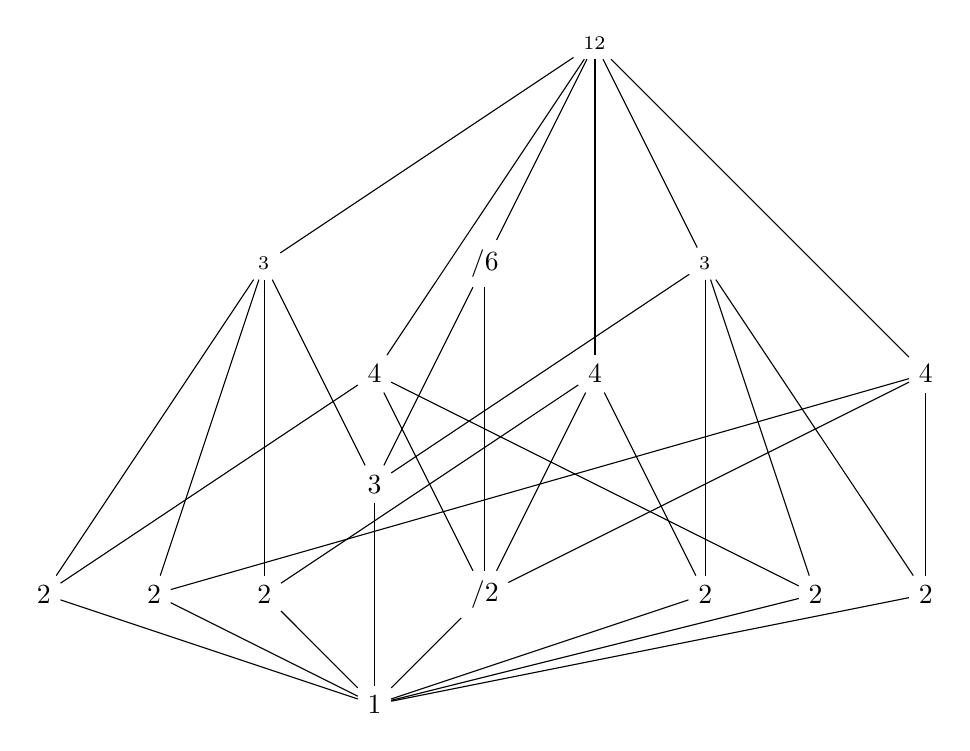
\begin{tikzpicture}[node distance=1.4cm]
\node (1) {$1$};
\node (d122) [above of = 1, left of = 1]{$2$};
\node (d132) [left of = d122]{$2$};
\node (d112) [left of = d132]{$2$};
\node (c2) [above of = 1, right of = 1]{$\Z/2\Z$};
\node (d222) [right of = c2, right of = c2]{$2$};
\node (d212) [right of = d222]{$2$};
\node (d1321) [right of = d212]{$2$};
\node (c3) [above of = 1, above of  = 1] {$3$};
\node (d14) [above of  = c3] {$4$};
\node (d24) [right of  = c2, above of = c2, above of = c2] {$4$};
\node (d34) [above of = d1321, above of = d1321] {$4$};
\node (c6) [above of  = c2, above of = c2, above of = c2] {$\Z/6\Z$};
\node (d16) [above of  = d122, above of = d122, above of = d122] {$\Sg_3$};
\node (d26) [above of  = d222, above of = d222, above of = d222] {$\Sg_3$};
\node (d12) [above of  = d24, above of = d24, above of = d24] {$\D_{12}$};
\draw (d34) -- (d1321);
\draw (1) -- (d112);
\draw (1) -- (d132);
\draw (1) -- (d122);
\draw (1) -- (c2);
\draw (1) -- (c3);
\draw (1) -- (d222);
\draw (1) -- (d212);
\draw (1) -- (d1321);
\draw (d112) -- (d16);
\draw (d132) -- (d16);
\draw (d122) -- (d16);
\draw (c3) -- (d16);
\draw (d12) -- (d16);
\draw (d112) -- (d14);
\draw (d14) -- (d212);
\draw (d14) -- (d12);
\draw (d14) -- (c2);
\draw (d24) -- (d122);
\draw (d24) -- (c2);
\draw (d24) -- (d222);
\draw (d24) -- (d12);
\draw (d34) -- (d132);
\draw (d34) -- (c2);
\draw (d34) -- (d12);
\draw (c6) -- (c3);
\draw (c6) -- (c2);
\draw (c6) -- (d12);
\draw (d26) -- (d1321);
\draw (d26) -- (d212);
\draw (d26) -- (d222);
\draw (d26) -- (c3);
\draw (d26) -- (d12);
\end{tikzpicture}
\end{center}
%(I said I wouldn't typeset the lattice of the binary dihedral group but I typeset that...)
\section{Automorphisms of cyclic groups}

\begin{definition}
An \defn{automorphism} is an isomorphism from a group $G$ to itself. The set of all automorphisms forms a group that is denoted $\Aut(G)$.
\end{definition}

The only group of order $13$ is $\Z/13\Z$, and the only groups of order $14$ are $\Z/14\Z$ and $\D_{14}$. To classify the groups of order $15$, we will consider groups $G$ of order $pq$ where $p<q$.

By \cref{cauchy}, $G$ has subgroups of order $p$ and $q$. The number of subgroups of order $q$ is $1\pmod q$ and divides $pq$, so this number must divide $p$. Since $p<q$, the number of subgroups of order $q$ is $1$, and this subgroup is normal in $G$. So $G$ is a semidirect product $\Z/q\Z \ltimes \Zmod p$. Determining how $\Zmod p$ can act on $\Zmod q$ will allow us to find all groups of order $pq$. 

An action of $\Zmod p$ on the group $\Zmod q$ is a homomorphism from $\Zmod p$ to $\Aut(\Zmod q)$. What are the automorphisms of $\Zmod q$? 

Well, what are the automorphisms of $\Zmod n$? The homomorphisms given by $1\mapsto g \in \Z/n\Z$ are automorphisms if $g$ is invertible in $(\Z/n\Z)^*$, that is, the multiplicative group of elements prime to $n$ or the units in the ring $\Z/n\Z$. 

Let's look at the first few cases. 
\begin{enumerate}
\item $(\Zmod n)^* = \{1\} \isomto \Z/1\Z$
\item $(\Zmod n)^* = \{1\} \isomto \Zmod 1$
\item $(\Zmod n)^* = \{1,2\}\isomto \Zmod 2$ where $2$ is a generator
\item $(\Zmod n)^* = \{1,3\}\isomto \Zmod 2$ where $3$ is a generator
\item $(\Zmod n)^* = \{1,2,3,4\}\isomto \Zmod 4$ where $2$ or $3$ are generators
\item $(\Zmod n)^* = \{1,5\}\isomto \Zmod2$ where $5$ is a generator
\item $(\Zmod n)^* = \{1,2,3,4,5,6\}\isomto \Zmod6$ where $3$ and $5$ are generators
\item $(\Zmod n)^* = \{1,3,5,7\}$ is not cyclic 
\item $(\Zmod n)^* = \{1,2,4,5,7,8\}\isomto \Zmod6$
\item $(\Zmod n)^* = \{1,3,7,9\}\isomto \Zmod4$ where $3$ and $7$ are generators
\item $(\Zmod n)^* = \{1,2,3,4,5,6,7,8,9,10\}\isomto \Zmod{10}$ where $2$ is a generator
\item $(\Zmod n)^* = \{1,5,7, 11\}$ is not cyclic
\end{enumerate}

\begin{proposition}
If $p$ is prime then $(\Zmod p)^*$ is cyclic of order $p-1$.
\end{proposition}


The ring $\Zmod p$ is a field. A polynomial of degree $n$ over a field has at most $n$ roots. So $(\Zmod p)^*$ has at most $n$ elements with $x^n = 1$. Also, the group $(\Zmod p)^*$ has at most $\varphi(n)$ elements of order $n$. Also, 
$$
\sum_{d\mid n} \varphi(d) = n.
$$
When $n=12$, we have $\Zmod n = \{0,1,2,3,4,5,6,7,8,9,10,11\}$, and we want will determine the order of each element. $1$ is the only element of order $1$, $6$ is the only element of order $2$, the elements of order $3$ are $4$ and $8$, $3$ and $9$ are the elements of order $4$, $2$ and $10$ are the elements of order $6$, and the elements of order $12$ are $1$, $5$, $7$, and $11$. The number of elements of order $2$ is $\varphi(2)$, the number of elements of order $3$ is $\varphi(3)$, and so on. 

Why? Let's consider the elements of order $4$, which are $3$ and $9$. Now, adding $0$ and $6$ into the mix, we get $ \{0,3,6,9\} = 3(\Zmod 4)$. The elements of order $4$ in $\Zmod{12}$ are just the elements of order $4$ in $3(\Zmod 4)$. Since $3(\Zmod 4)$ has $\varphi(4) $ elements, so does $\Zmod {12}$. So, 
$$
\varphi (1) + \varphi (2)  + \varphi (3) + \varphi (4) + \varphi (6) + \varphi (12) = 12.
$$
Convince yourself that this works for all other $n$.

The group $G = (\Zmod p)^*$ is abelian and has at most $\varphi (n) $ elements of order $n$. For all $n$ dividing $\abs{G}$, $G$ has at most $\varphi(n)$ elements of order $n$. Also, $\sum_{n \textrm{ dividing } \abs{G}} \varphi(n) = \abs{G}$. So $G$ has $\varphi(n)$ elements of order $n$, and $G$ has some elements with order $\abs{G}$. Therefore $G$ is cyclic, and a generator of this group is sometimes called a \defn{primitive root}.

Okay. Back to classifying groups of order $pq$. We know that a group $G$ of order $pq$ is the semidirect product $\Z/q\Z \ltimes \Zmod p$. We want to find out all ways $\Zmod p$ can act on $\Zmod q$. The group of automorphisms of $\Zmod q$ is $(\Zmod q)^* \isomto \Z/(q-1)\Z$, so we want to find maps from $\Z/p\Z$ to $\Z/(q-1)\Z$.

There are no homomorphisms other than $0$ unless $p$ divides $q-1$, and if it does, then we get some homomorphisms that are all sort of equivalent under automorphisms of $\Z/p\Z$. So we have a nontrivial semidirect product $\Z/q\Z \ltimes \Z/p\Z$ unique up to isomorphism. 

In summary, there is one group up to isomorphism of order $pq$ with $p<q$ if $p$ does not divide $q-1$ and two groups up to isomorphism if $p$ divides $q-1$. So, if $\abs{G} = 15$, then $G \isomto \Z/15\Z$. We can see that if $p=2$, then we get two groups that we know are isomorphic to either $\Z/2q\Z$ or $\D_{2q}$.

Let's discuss the structure of the group $(\Zmod n)^*$ for $n$ composite. We proceed for the remainder of this section without proof, so it is a good idea to prove everything that is not transpicuous to you. (And that's always a good idea, Jack.) If $n = p_1^{a_1} p_2^{a_2}\cdots $ then 
$$
(\Zmod n)^* \isomto \prod_i (\Z/p_i^{a_i}\Z)^*.
$$
So, we assume $n$ is a prime power. The group $(\Zmod {p^f})^*$ is cyclic of order $\varphi (p^f) = p^{f-1} (p-1)$ unless $p=2$, when 
$$
(\Zmod {p^f})^* \isomto \Zmod 2 \times \Zmod {2^{f-2}}
$$
where the first group is generated by $\pm 1$ and the second is the powers of $5$. When $p\ne 2$, we have 
$$
(\Zmod {p^f})^* \isomto \Zmod {p^{f-1}} \times \Zmod {(p-1)},
$$
where the first group is generated by $p+1$.

Why do things go wrong when $p=2$? We want to show that $1+p$ has order $p^{f-1}$ in $(\Zmod {p^f})^*$, and you start by showing that $(1+p)^{p^{f-2}}\ne 1$ in $(\Zmod {p^f})^*$. This is a good exercise.

\begin{exercise}
Suppose $p\ne 2$ is prime. Show that 
$$
(\Zmod {p^f})^* \isomto (\Zmod {p^{f-1}}) \times (\Zmod {(p-1)}).
$$
\end{exercise}

But it fails when $p=2$. We have
\begin{align*}
(1+p)^{p^{f-2}} &= 1 + p^{f-2} p + \binom{p^{f-2}}{2} p^2 + \binom{p^{f-2}}{3} p^3 + \cdots\\
&= 1 + p^{f-1} + \binom{p^{f-2}}{2} p^2 + \cdots
\end{align*}
When $p\ne 2$, the terms after $p^{f-1}$ are divisible by $p^f$, so that whole sum is not $1\pmod {p^f}$. However, when $p=2$, not all of these terms are divisible by $p$ (the third term), so we can't guarantee that the sum is not $1\pmod {p^f}$.
\begin{example}
We have
$$
(\Zmod {1000000})^* \isomto (\Zmod {2^6})^* \times (\Z/5^6\Z)^*
$$
by the Chinese remainder theorem, so
$$
(\Zmod {1000000})^* \isomto (\Zmod {2}) \times (\Z/2^4\Z) \times (\Zmod {5^5}) \times (\Zmod {2^2}).
$$
\end{example}

\section{Finite abelian groups}
Let's start with classifying abelian groups of order $16$. We have $\Zmod{16}$, $\Zmod 8\times \Zmod 2$, $\Zmod 4 \times \Zmod 4$, $\Zmod 4 \times \Zmod 2\times\Zmod 2$, and $\Zmod 2 \times \Zmod 2\times \Zmod 2\times \Zmod 2$. 

When considering abelian groups we have seen previously, we notice they have been products of cyclic groups. It's not true that every abelian group can be written as the product of cyclic groups; for instance, $\Q $ under addition is not a product of cyclic groups.

\begin{theorem}\label{decomp}
Every finitely generated abelian group $G$ is a direct sum of groups $\Z/p^f\Z$ and $\Z$.
\end{theorem}
More generally, any finitely generated module over a Euclidean domain $R$ is a sum of cyclic modules $R/aR$.
\begin{proof}
Suppose $g_1 ,\cdots,g_k$ are generators with enough relations
\begin{align*}
n_{11}g_1 + \cdots + n_{1k} g_k &= 0\\
n_{21} g_1 + \cdots + n_{2k} g_k&=0\quad \mathrm{etc.}
\end{align*}
to specify the group $G$, which we write as a matrix. What can we do to this matrix without changing the group? We can add a multiple of one column to another, since if $g$ and $h$ are generators, then we can change these to $g+nh$ and $h$ for an integer $n$. We can also add a multiple of a row to another, since if $R_1$ and $R_2$ are relations, then $R_1$, $R_2+nR_1$ are equivalent relations.

We perform these operations to minimize $n_{11}$ in absolute value, and then subtract multiples of the first row and column from the others to make all entries $n_{12}, n_{13},\hdots,n_{21}, n_{31} ,\hdots$ equal to $0$. We can do this because $n_{12}$ must be a multiple of $n_{11}$. We repeat this process on the resulting submatrix until the matrix of relations is diagonal.

We conclude that the group has generators $g_1,\hdots,g_k$ with relations $n_{ii} g_i = 0$, so the group is isomorphic to a product of cyclic groups of order $n_{ii}$ that decompose into cyclic groups of prime power order. If $n_{ii} = 0$, then $\Z/n_{ii}\Z \isomto \Z$.
\end{proof}

When are two finite abelian groups isomorphic? Suppose 
$$
G \isomto \Z/p_1^{n_1}\Z \times \Z /p_2^{n_2}\Z \times \cdots.
$$
Do the $p_i,n_i$ determine the group (up to reordering)? (It turns out they do.) % if we have $\Z/p_1^{n_1}\Z \times \Z/p_1^{n_2}\Z \times \Z/p_1 ^{n_3}\Z \times\cdots$, then the number of times $p_1^f$ occurs is determined by the number of elements of order $p_1$ in $G$. Similarly, the number of elements of order $p^2$ determines the number of times we get $p^{2+f}$ in the denominator. So

How many abelian groups are there of order $p^f$? If we write $f = \sum_i \alpha_i $ with $\alpha_1\ge \alpha_2\ge \alpha_3 \ge \cdots > 0$, then we get a group
$$
\Zmod{p^{\alpha_1}} \times \Zmod{p^{\alpha_2}} \times \Zmod{p^{\alpha_3}}  \times \cdots. 
$$
So the number of groups is the number of partitions of $f$. (Partitions are super cool.)

There is a close correspondence between \cref{decomp} and the following theorem.
\begin{theorem}\label{cjnf}
Every matrix over the complex numbers has Jordan normal form. 
\end{theorem}
How are they related? \cref{decomp} works for modules over $\Z$, and \cref{cjnf} works for modules over $\C[x]$. A \defn{module} is a vector space where the scalars form a ring, not necessarily a field. It is a vector space with a linear transformation (which is the action of $x$). Finite abelian groups are sums of cyclic groups, and the corresponding theorem for modules over polynomial rings says that if $p = (x-\alpha)$ is an irreducible polynomial then $\C[x] / p^f \C[x] $ (where  $(x-\alpha)^f=1$) gives a basis
$$
\mat{\alpha &1&  & \\ & \alpha& \ddots&   \\ &  & \ddots & 1 \\  &   &  & \alpha} 
$$
with $f$ rows. 

\section{Nilpotent groups}
Let's list the groups of order $16$. There are $p(4) = 5$ abelian groups, namely 
\begin{enumerate}
\item $\Zmod {16}$, 
\item $\Zmod{8} \times \Zmod 2$, 
\item $\Zmod 4 \times \Zmod 4$, 
\item $\Zmod 4 \times \Zmod 2 \times \Zmod 2$, and 
\item $\Zmod 2 \times \Zmod 2 \times \Zmod 2 \times \Zmod 2$.
\end{enumerate}
We also have $2$ products $\Z/2\Z \times \D_8$ and $\Z/2\Z \times \Qu$, and $4$ non-abelian groups with an element of order $8$, namely
\begin{enumerate}
\item the generalized quaternion group (the binary dihedral group of order $16$) and
\item three groups of the form $\Zmod 8 \ltimes \Zmod 2$ where if $a^8 = 1$ and $b^2=1$, then $bab\inv = a^3,a^5,a^7$. The group with $bab\inv = a^7$ corresponds to $\D_{16}$ and the $a^3$ group is called the semidihedral group.
\end{enumerate}
We also have various semidirect products:
\begin{enumerate}
\item $\Zmod 4\ltimes \Zmod 4$,
\item $(\Zmod 2\times \Zmod 2) \ltimes \Zmod 4$, and
\item $(\Zmod 4 \times \Zmod 2) \ltimes \Zmod 2$, the \defn{Pauli group} on one qubit.
\end{enumerate}

Recall \cref{nilp}. 
\begin{proof}
All conjugacy classes have order a power of $p$, so the size is $1$ or divisible by $p$. So the number of conjugacy classes of size $1$ is divisible by $p$. A conjugacy class of size $1$ is an element of the centre, so we can mod out by the centre. The result follows by induction. 
\end{proof}
So all groups $G$ of order $16$ are nilpotent.
\begin{proposition}
The product of $2$ nilpotent groups is nilpotent. 
\end{proposition}
\begin{proof}
``Easy.''
\end{proof}
\begin{proposition}
The following are equivalent for finite groups. 
\begin{enumerate}
\item A group $G$ is a product of $p$-groups,
\item $G$ is nilpotent, and
\item all Sylow subgroups of $G$ are normal (there at most $1$ Sylow $p$-subgroup for any $p$).
\end{enumerate}
\end{proposition}
%\begin{proof}
%($G$ is nilpotent $\implies$ Sylow subgroups are normal.) By induction on $\abs{G}$. Pick $g\in \ZZ(G)$ with $g^p=1$. (We can do this since $G$ is nilpotent.) The group $G / \ang g$ is still nilpotent, so all Sylow subgroups of $G/\ang g$ are nilpotent. Suppose $q=p$. Then the Sylow $q$-subgroup of $G/\ang g$ is normal so the inverse image in $G$ is a Sylow $p$-subgroup of $G$. Suppose $q\ne p$. Pick the Sylow $q$-subgroup of $G/ \ang g$ and consider the inverse image in $G$. The inverse image has order $pq^f$ for some $f$. The Sylow subgroup of order $q^f$ must be normal since its only conjugates would be in the centre. So the Sylow $q$-subgroup is unique. % confusing
%\end{proof}
%
%\begin{proof}
%(Sylow subgroups are normal $\implies G$ is a product of $p$-groups.) Pick a Sylow $p$-subgroup $P$ and a Sylow $q$-subgroup $Q$ where $p\ne q$. The subgroups $P$ and $Q$ commute. 
%\begin{proof}[Proof for proof]
%Suppose $a\in P, b\in Q$. Since $Q$ is normal, $aba\inv \in Q$, so $aba\inv b\inv \in Q$. Also, $ba\inv b\inv\in P$ since $P$ is normal, so $aba\inv b\inv \in P\cap Q$. But $P\cap Q$ is trivial, so $aba\inv b\inv  =1$, so $ab=ba$.
%\end{proof} 
%There is a Sylow subgroup for every prime $p$ and they all commute, so the group is a product of them.
%\end{proof}

\section{Wreath products}
Let's look at groups $G$ of order $18$. By \cref{Sylow} $G$ has a subgroup of order $9$. Since it has index $2$, it is normal, so $G$ is a semidirect product of a group of order $9$ with $\Z/2\Z$. We know that the subgroup of order $9$ is either $\Z/9\Z$ or $(\Zmod 3) \times (\Zmod 3)$.

If the subgroup is $\Zmod 9$, the group of order $2$ can act as $1$, which corresponds to $\Z/18\Z$, or $-1$, which corresponds to $\D_{18}$.

 If the subgroup is $(\Zmod 3) \times (\Zmod 3)$, we have to consider how $\Zmod 2$ can act on it. The subgroup is a vector space $V$ of dimension $2$ over $\F_3$. The nontrivial element of $\Z/2\Z$ is an order $2$ linear transformation $\sigma$. The vector space $V = V_1 \oplus V_2$ is the sum of eigenspaces of $\sigma$ where $\sigma = 1$ on $V_1$ and $\sigma =-1$ on $V_2$. The space $V_1$ can have dimension $2,1$, or $0$, so, in total, we have
$$
\sigma = \mat{1 & \\ & 1},\mat{1 & \\ & -1},\mat{-1 & \\ & -1}
$$ 
corresponding to the $3$ conjugacy classes of linear transformations of order $2$ over $V$. This gives us $3$ possibilities for $G$. The first one gives $(\Zmod3 \times \Zmod 3)\times \Zmod 2$, the second gives $\Zmod 3 \times \Sg_3$, and the last gives $(\Zmod 3 \times \Zmod 3)\ltimes \Zmod 2$. This last one is an example of a Frobenius group, and the second one is an example of a {wreath product}.
\begin{definition}
A \defn{wreath product} of $G$ and $H$ is given by
$$
G\wr H = \left (\underbrace{G \times G \times \cdots \times G}_{\abs{H} \textrm{ times}}\right)\ltimes H.
$$
%The group $H$ acts on the product by its regular representation, so $H$ acts on itself by left translations.
\end{definition}

\begin{example}\text{}
\begin{enumerate}
\item Take $G=\Zmod 3$ and $H = \Zmod 2$. Then 
$
G\wr H = ((\Zmod 3) \times (\Zmod 3)) \ltimes \Zmod 2
$ 
where $\Zmod 2$ acts by flipping the two groups of order $3$.
\item $\D_8 = \Z/2\Z \wr \Z/2\Z$.
\item Automorphisms of trees are often wreath products. \iffalse Suppose we have the tree $T$
%\begin{center}
%\begin{tikzpicture}[sibling distance = 0.2cm, level distance = 1cm]
% 
%\node(t)  [dot]
%    child [anchor = east] {[fill] circle (2pt)
%    child {[fill] circle (2pt)}
%    child {[fill] circle (2pt)}
%    child {[fill] circle (2pt)}
%    child {[fill] circle (2pt)}}
%    child [anchor = west] {[fill] circle (2pt)
%    child {[fill] circle (2pt)}
%    child {[fill] circle (2pt)}
%    child {[fill] circle (2pt)}
%    child {[fill] circle (2pt)}};
%\end{tikzpicture}
%\end{center}
\begin{center}
\includegraphics [scale = 0.5] {images/thing2.png}
\end{center}
Then $\Aut(T) = \Sg_4 \wr \Sg_3$.\fi
\end{enumerate}
\end{example} %mobiles? really?

Wreath products also show up in the Sylow subgroups of symmetric groups. For symmetric groups of index $p^f$ you get an $f$-fold wreath product of $\Z/p\Z$, a sort of tower of wreath products. For instance, if $G=\Sg_{27}$, then we get $((\Z/3\Z )\wr (\Z/3\Z)) \wr (\Z/3\Z)$. For others you get products of these towers. See lecture 19 around minute 11 for more detail. % 11:10 (https://www.youtube.com/watch?v=2Ik9m84AT2E&list=PL8yHsr3EFj51pjBvvCPipgAT3SYpIiIsJ&index=19) 

%Suppose $H$ acts on $S$. Then we have
%$$
%\left (\underbrace{G \times G \times \cdots \times G}_{\abs{S} \textrm{ times}}\right)\ltimes H = G^S \ltimes H
%$$
%where $G^S$ is all functions from $S$ to $G$ (or all continuous functions). Take $S$ spacetime, $H$ symmetries of spacetime, and $G$ a gauge group, for instance $S^1$. Then $G^S$ is all functions from spacetime to $S^1$. 
\section{Frobenius groups}
Let's consider groups of order $20$. We know there is a Sylow subgroup of order $5$ that is normal, so $G$ is a semidirect product of $\Z/5\Z$ with a group of order $4$. We know $\Aut(\Z/5\Z) \isomto \Z/4\Z$. If the group of order $4$ is $(\Zmod 2)\times(\Zmod 2)$, there are two possibilities. If the action is trivial, then we get $\Z/5\Z \times \Z/2\Z \times \Z/2\Z$. If it's nontrivial, we get $\D_{10}\times\Zmod 2$. If the group of order $4$ is $\Zmod 4$, we have $3$ possibilities. If the action is trivial, we get $\Zmod{20}$. If $\Z/4\Z$ acts as a group of order $2$ on $\Zmod 5$, we get a semidirect product $\Z/5\Z\ltimes \Z/4\Z$ which is the binary dihedral group of order $20$. We also get $\Z/5\Z\ltimes \Z/4\Z$ which is the $ax+b$ group.

This last group is a Frobenius group.
\begin{definition}
A \defn{Frobenius group} $G$ is a group acting transitively on a set $S$ such that no nonidentity element of $G$ fixes at least two elements of $S$ and $S$ is not the regular representation.
\end{definition}

\begin{example}\text{}
\begin{enumerate}
\item The $ax+b$ group over a field $F$ is Frobenius, where $S$ consists of elements in $F$, $a\in F^*$, and $b\in F$, with order $\abs{F} (\abs{F} - 1)$.
\item The group $\D_n$ for $n$ odd is Frobenius.
\item The group $(\Z/3\Z)^2 \ltimes \Z/2\Z$ is Frobenius.
\end{enumerate}
\end{example}

\begin{definition}
A subgroup $H\ne \{1\}$ of a finite group $G$ is called a \defn{Frobenius}  \\\defn{complement} if $H\cap H^g = \{1\}$ for all $g\in G\setminus H$. The \defn{Frobenius kernel} is
$$
K = \left(G \setminus \bigcup_{g\in G} H^g \right)\cup \{1\}.
$$
\end{definition}


\begin{theorem}[Frobenius]\label{frob}
%Let $G$ be a group. Let $H$ be the subgroup fixing a point and $K$ all conjugates (all elements not in a conjugate of $H$ with $1$). Then $K$ is a normal subgroup and $G = K\ltimes H$, where $K$ is called the \defn{Frobenius kernel}.
Let $G$ be a finite group, $H$ a Frobenius complement of $G$, and $K$ the corresponding Frobenius kernel. Then $K$ is a normal subgroup in $G$ and 
$$
G = K\ltimes H.
$$
\end{theorem}

\begin{proof}
Uses character theory,\footnote{See \url{https://terrytao.wordpress.com/2013/05/24/a-fourier-analytic-proof-of-frobeniuss-theorem/}.} so skipped.
\end{proof}

\begin{theorem}[Thompson]\label{thom}
The Frobenius kernel $K$ is nilpotent.
\end{theorem}
\begin{example}
Take 
$$
K = \mat{ 1 & * & * \\ 0 &1 &*\\ 0&0&1} \in \GL_3({\F_7})
$$
and 
$$
H = \left \langle \mat{ 1 & 0&0  \\ 0 &2 &0\\ 0&0&4}\right \rangle .
$$
Then $KH $ is a Frobenius group of order $7^3\cdot 3$.
\end{example}

There are two possibilities for groups of order $21$: $\Z/21\Z$ and $\Z/7\Z\ltimes \Z/3\Z$. The second group is a Frobenius group. We know groups of order $22$ are either $\Z/22\Z$ or $\D_{22}$, and the only group of order $23$ is $\Z/23\Z$.

\section{Groups of order $24$}
There are $15$ groups of order $24$. There's a Sylow $3$-subgroup, and there might be one such subgroup or $4$ subgroups. 

Let's look at the case when $G$ has one normal Sylow $3$ subgroup. Then $G$ is a semidirect product of $\Zmod 3$ with a group of order $8$ (the Sylow $2$-subgroup). The Sylow $2$-subgroup can be $\Zmod 8$, $\Zmod 4\times \Zmod 2$, $(\Zmod 2)^3$, $\Qu$, or $\D_8$. What is the action of the group of order $8$ on the group of order $3$? We have $\Aut(\Zmod 3) \isomto \Zmod 2$. 

The action on $\Zmod 3$ can be trivial or nontrivial. If the action is trivial, then $G$ is a direct product of $\Zmod 3$ with the mentioned groups of order $8$. If the action is nontrivial, then we get two groups from $\Zmod 4\times \Zmod 2$ and $\D_8$, and $1$ from each of the other groups of order $8$. We have two groups for these two groups of order $8$ because kernel of the map from either $\Zmod 4\times \Zmod 2$ or $\D_8$ to the group of order $3$ can be cyclic or a direct product of two cyclic groups.

Now suppose we have $4$ Sylow $3$-subgroups (not normal). So $G$ acts by conjugation on these four Sylow $3$-subgroups.  $G$ acts transitively, so we get a homomorphism from $G$ to $\Sg_4$ (the permutations of the Sylow subgroups). What is the kernel of this homomorphism? The kernel must have order dividing $6$ because we have a transitive action of $G$ on a set of $4$ elements. The kernel cannot have order $3$ or $6$, since the order $3$ subgroup of the kernel would be normal in $G$. If the kernel has order $1$, then $G\isomto\Sg_4$. 

If the kernel has order $2$, the image has order $12$ and has more than $1$ Sylow $3$-subgroup (otherwise, $G$ would have a normal Sylow $3$-subgroup), so $G\isomto \Ag_4$. The group $\Ag_4$ has a normal subgroup of order $2$, and its preimage in $G$ is a normal subgroup of order $8$, so, in this case, $G$ has a normal subgroup of order $8$, meaning $G$ is the semidirect product of a group of order $8$ with a group of order $3$ (with nontrivial action). There are two possibilities here: $(\Zmod 2)^3\ltimes \Zmod 3$ or $\Qu \ltimes \Zmod 3$. The first case gives $\Ag_4 \times \Zmod 2$, and the other gives the binary tetrahedral group.

%So we have found $3$ ways to ``join'' $\Ag_4$ with $\Zmod 2$.
Let's consider the binary tetrahedral group. Recall that the group $S^3$ of unit quaternions maps to $\SO_3(\R)$. Inside $\SO_3(\R)$ is $\Ag_4$ (the rotations of the tetrahedron). We have the following \defn{central extension}
$$
1 \longrightarrow \Zmod 2 \longrightarrow \widehat{\Ag_4} \longrightarrow \Ag_4 \longrightarrow 1 
$$
where $\widehat{\Ag_4}$ denotes the binary tetrahedral group. 

The ring of \defn{Hurwitz quaternions}
$$
H = \{ a+ bi + cj + dk : a,b,c,d \in \Z \textrm{ or } a,b,c,d \in (\Z + 1/2)\} 
$$
has units $\pm 1,\pm i ,\pm j, \pm k$, and all quaternions of the form $(\pm 1 \pm i \pm j \pm k)/2$. These units form the binary tetrahedral group.

The group $\Sg_4$ doesn't have very many normal subgroups. It has $\{1\} \subset \Zmod 2 \times \Zmod 2\subset \Ag_4 \subset \Sg_4$. The group $\Sg_4$ is the first group with no normal Sylow subgroups.
\begin{definition}
A group $G$ is \defn{solvable} if we can find a series of subgroups
$$
\{1\} = G_0 \subset G_1 \subset \cdots \subset G_n = G
$$
such that $G_i$ is normal in $G_{i+1}$ and $G_{i+1} / G_i$ is cyclic of prime order.
\end{definition}

All nilpotent groups are solvable. The smallest group that is not solvable is $\Ag_5$. 

The quotient of $\Sg_4$ by $\Zmod 2\times \Zmod 2$ gives a homomorphism from $\Sg_4 $ to $ \Sg_3$. Suppose we have $4$ points acted on by $\Sg_4$. We can construct a set of $3$ things acted on by $\Sg_3$ by taking all ways we can join the four points in pairs. Any permutation of the four points gives a permutation of these three objects.
\section{Symmetric groups}
The symmetric group $\Sg_n$ is the group of permutations of $n$ letters, where
$$
\abs{\Sg_n} = n!%\frac{e^{-\gamma (n+1)}}{n+1} \prod_1^\infty \left(1 + \frac{n+1}{k}\right)\inv e^{(n+1)/k} % nice
$$ 
%(where $\gamma$ is the Euler-Mascheroni constant). 
It has a subgroup $\Ag_n$, the alternating group, with index $2$, and $\abs{\Ag_n} = n!/2$ if $n>1$. The group $\Ag_n$ consists of the permutations fixing 
$$
\prod_{0<i<j\le n} (x_i - x_j).
$$
Indeed, we have a homomorphism $\Sg_n \longrightarrow \{\pm 1\}$ where the sign depends on the sign of the above polynomial. The group $\Ag_n$ is the kernel of this homomorphism, so we have the exact sequence
$$
1 \longrightarrow \Ag_n \longrightarrow \Sg_n \longrightarrow \{\pm 1\} \longrightarrow 1.
$$
The group $\Ag_n$ is normal in $\Sg_n$ because it is the kernel of a homomorphism.

The groups $\Sg_1$ and $\Ag_1$ are trivial. The group $\Sg_2$ is cyclic of order $2$ and $\Ag_2$ is trivial. The group $\Sg_3\isomto \D_6$ is the first nonabelian group, and $\Ag_3\isomto \Zmod 3$. We have 
$$\Sg_4 \rhd \Ag_4 \rhd (\Zmod2\times \Zmod 2) \rhd \{1\},$$ which is the only case when a symmetric group has a nontrivial normal subgroup other than the alternating group. The group $\Ag_4$ is also the rotations of a tetrahedron, and the group $\Sg_4$ is the rotations of a cube or octahedron. 
\begin{definition}
A group $G$ is a \defn{simple group} if its only normal subgroups are $\{1\}$ and $G$.
\end{definition}

The group $\Ag_5$ is the rotations of an icosahedron; the group $\Ag_5$ is the first nonabelian simple group, and the first that isn't cyclic of prime order. The group $\Sg_6$ has nontrivial automorphisms of an unexpected form.

The conjugacy classes of $\Sg_n$ are easy to describe. Any element of $\Sg_n$ is a product of disjoint cycles, and conjugating a permutation preserves its cycle shape. Conversely, any two elements of the same cycle shape are conjugate. Suppose that
$a = (1\ 2\ 3)(4\ 5)(6\ 7)$, $b = (6\ 4\ 3)(2\ 1)(7\ 5)$, and we want to determine $g$ such that $gag\inv =b$. We find that $g$ can be the permutation mapping $1$ to $6$, $2$ to $4$, $3$ to itself, $4$ to $2$, etc. So $g = (1\ 6\ 7\ 5)(2\ 4)(3)$. This $g$ is not unique.

So the conjugacy classes of $\Sg_n$ correspond to cycle shapes of length $n$, and the number of conjugacy classes of $\Sg_n$ is $p(n)$. (Partitions again. Yay!)

So what are the conjugacy classes of $\Sg_4$? We can write $4 = 4 = 3+1 = 2+2 = 2+1 + 1 = 1+1+1+1$ where each partition corresponds to a conjugacy class. 

How many elements are in each conjugacy class? The size of the conjugacy class is the size of the orbit under $G$, which is $\abs{G}$ divided by the order of the subgroup fixing a point, which is the order of the subgroup commuting with one permutation. If we have a permutation with cycle shape $(1^3)( 2^2 )(3^1)(4^2)$, then it commutes with a group of order $1^3 \times 3! \times 2^2 \times 2!\times 3^1 \times 1! \times 4^2 \times 2!$ So the order of the centralizer of a permutation of shape $\prod_ i i^{n_i}$ is $\prod_i i^{n_i} n_i!$, so the size of the conjugacy class is
$$
\frac{n!}{\prod_i i^{n_i} n_i!}
$$

Conjugacy classes in $\Ag_n$ are similar, but classes of $\Sg_n$ sometimes split into $2$ classes of $\Ag_n$. Take, for example, $\Ag_3$. The set of conjugacy classes of $\Sg_3$ is 
$$
\{\{1\}, \{(1\ 2\ 3), (1\ 3\ 2)\}, \{(1\ 2),(2\ 3),(3\ 1)\}\}.
$$
The $2$-cycles are not elements of $\Ag_3$, but $\Ag_3$ has $3$ conjugacy classes; that is, the second conjugacy class of $\Sg_3$ split into two conjugacy classes in $\Ag_3$. The problem is that the element conjugating the one $3$-cycle to the other is a $2$-cycle (not in $\Ag_3$). We have a similar thing with $\Ag_4 \subset \Sg_4$. However, $\Ag_5\subset \Sg_5$ doesn't have this problem (the $3$-cycles form one conjugacy class in $\Ag_5$.) We can conjugate the first $3$-cycle to the second by the permutation $(2\ 3)\notin \Ag_5$. We multiply by $(4\ 5)$ to get the element into the alternating group. There is an algorithm for determining whether $\Ag_n$ does this, but Dr. Borcherds is forgetful, so you will never find out.

What are the generators of $\Sg_n$? The generators are the transpositions (an element swapping two letters). We want to show that every permutation is a product of transpositions. 

``We use the notorious bubble sort. . . . Anyway, fortunately, bubble sort has been more or less eradicated from computing, but it's still very useful in the theory of the symmetric group.''

\section{Coxeter-Todd algorithm}
The symmetric group is generated by the transpositions. What are the relations between the transpositions? Of course, if $\tau$ is any transposition, then $\tau^2 = 1$. If $\tau_1 = (\alpha_1\  \alpha_2)$ and $\tau_2 = (\alpha_2\ \alpha_3)$, then $(\tau_1\tau_2)^3=1$. If $\tau_3 = (\alpha_3\ \alpha_4)$, then $(\tau_1\tau_3)^2=1$.

Coxeter came up with a compact way of writing relations like these: \defn{Coxeter diagrams}. The Coxeter diagram for $\Sg_n$ is 
$$
\Sg_n : \underbrace{\dynkin [Coxeter]A{}}_{n-1 \textrm{ points}}
$$
For each point $\tau$, $\tau^2=1$. If $\tau$ is connected to $\tau'$, then $(\tau\tau')^3 = 1$. If $\tau$ is not connected to $\tau'$, then $(\tau\tau')^2=1$.

Are there any other relations that we can't get from the previous ones? That is, do the relations above define the symmetric group? Suppose $G$ is a group defined by these relations. Then there is a map $G\longrightarrow \Sg_n$ that is surjective because $\Sg_n$ is generated by the relations. We want to show that the kernel of this map is $\{1\}$ such that the $G$ is isomorphic to $\Sg_n$. It is enough to show that $\abs{G} \le \abs{\Sg_n}$. 

Suppose we have the Coxeter diagram
$$
G : \dynkin [Coxeter]A{4}
$$
Label the points $\alpha_1,\alpha_2,\alpha_3,\alpha_4$. The group $G$ has a subgroup $H=\langle \alpha_1,\alpha_2,\alpha_3\rangle$, and, by induction, $\abs{H} \le \abs{\Sg_4}$. We want to show $\abs G / \abs H \le 5$. Construct the permutation representation on cosets of $H$ by brute force. This will be an action of $G$ on a set containing a point fixed by $H$. We write down the representation and find that $\abs{G} / \abs H = 5$. So $\abs{G} \le 5\abs H \le 120$, so $G\isomto \Sg_5$.

Dr. Borcherds shows the algorithm in action in his lecture.

\section{Extra special groups}
We will explore some analogues of the Heisenberg group, called extra special groups. Let's consider groups of order $25$, $26$, $27$, $28$, and $29$. There are only two groups of order $25$ are $\Zmod {25}$ and $\Zmod 5\times \Zmod 5$. A group of order $26$ is either $\Zmod{26}$ or $\D_{26}$. A group of order $29$ is cyclic.  The groups of order $28$ are similar to those of order $20$: we get two abelian groups, a dihedral group, and a binary dihedral group.  To classify the groups of order $27$, we will classify the groups of order $p^3$.

We have $3$ abelian groups of order $p^3$: $\Zmod{p^3}$, $\Zmod {p^2}\times \Zmod p$, and $(\Zmod{p})^3$. It turns out that there are two nonabelian groups. The group can have elements of order $p^2$, or all elements have order $1$ or $p$. If $p=2$, both $\D_8$ and $\Qu$ have elements of order $p^2$, and there are no groups such that all elements have order $2$ (otherwise the group would be abelian: $ab = (bb)ab(aa) = b (ba)(ba)a = ba$).

If $p$ is odd, then we have one nonabelian group for each case. Let $G$ be the group. If $G$ has an element of order $p^2$, the centre $Z$ is cyclic of order $p$. Then $G/Z = (\Zmod p)^2$, and we have the extension
$$
\{1\} \longrightarrow \Zmod p \longrightarrow G \longrightarrow (\Zmod p)^2 \longrightarrow \{1\}.
$$

First let's look at the case when all elements of $G$ have order $1$ or $p$. The group
$$
G=\left \{ \mat{  \,1 & \,* & \,*\, \\ \, & \,1 &\, *\,\\ \, & \, & \,1\, } \right\} \subset \GL_3(\F_p)
$$ 
is nonabelian of order $p^3$. Do all of its elements have order $p$, and, if so, why does that fail when $p=2$? We define the map
$$
\exp : \left \{ \mat{  \,\,& * & *\, \\ \, &  & *\,\\ \, &  & \, } \right\} \longrightarrow G,
$$
which, in this case, can be defined
$$
\exp : a \mapsto 1 + a + a^2/2.
$$
Also, $\log(1+a) = a - a^2/2$. (Notice that $a^3 = 0$ here.) We have $\exp (a+b)  = (\exp a)(\exp b)$ if $ab=ba$, so $\exp (na)= (\exp a)^n$. In the group, we have $g^p = \exp (p\log g) = 1$ since $p\log g=0$ in $\F_p$. All elements of $G$ have order $p$ except when $p=2$, since we're dividing by $2$ in $\exp$ and $\log$. If $p=2$, we have $G = \D_8$. 

We can check that there is only one such group. Any nonabelian group $G$ of order $p^3$ with $g^p = 1$ for all $g$ must be a semidirect product $(\Zmod p \times \Zmod p)\ltimes \Zmod p$. The automorphisms of the former group in the semidirect product are two-by-two matrices, and the automorphisms of order $p$ are conjugate to the automorphism $\mat{1 & 1 \\ &1}$. We might as well take a generator of $\Zmod p$ to act on the two-dimensional vector space by that automorphism. So the group has elements $a^p=1, b^p =1$ with $ab=ba$. Take $c \in \Zmod p$, so $c$ commutes with $a$ and $cb = abc$. We can check the generators define a group of order $p^3$ unique up to isomorphism. (That is, there is one nonabelian group of order $p^3$ where all nontrivial elements have order $p$ up to isomorphism.)

Suppose $G$ is nonabelian of order $p^3$ with an element of order $p^2$. The group $G$ has a normal subgroup $\Zmod {p^2} $ generated by $a : a^{p^2}= 1$. Pick $b \notin (\Zmod {p^2})$. The element $b$ must act nontrivially on $a$ (otherwise the group would be abelian). We choose $b$ such that $bab\inv = a^{1+p}$ which is always possible. We must have $b^p=1,a^p,a^{p^2},\hdots$. If $b^p=1$, then $G = (\Zmod{p^2})\ltimes (\Zmod p)$. If $p=2$, then the case $b^p = a^p $ gives a different group (the quaternion group) than the case $b^p = 1 $ (the dihedral group). If $p$ is odd, we can change $b$ to $c=ba$ where $cac\inv = a^{1+p}$. What is $c^p$ now? We have $c^p = (ba)^p = ba\cdots ba = a^{(p(p+1)/2)p}a^pb^p$. If $p\ne 2$, then the first term in $c^p$ is $a^{p^2(p+1)/2} = 1$, so $c^p = a^pb^p$. If $b^p = a^{np}$ is a power of $a$, then we get $c^p = a^{(n+1)p}$, and repeatedly doing this will give an element $d^{p} = 1$, so our group has relations $a^{p^2} = 1$, $dad\inv = a^{1+p}$, thus the group is a semidirect product.

So we only get $2$ nonabelian groups of order $p^3$. We can construct them by either taking the upper triangular matrices above or a semidirect product $\Zmod {p^2} \ltimes \Zmod p$. The first kind forms a family for all $p$, and the second forms a family for $p$ odd. When $p=2$, it turns out that one semidirect product is isomorphic to the group in matrix form (the dihedral group), and another semidirect product is isomorphic to $\Qu$. 

These groups are analogues of the Heisenberg group. Suppose $f:\R\longrightarrow\C$. We can transform $f$ by $T_\alpha : f(x)\mapsto f(x+\alpha)$ and $T_\beta : f(x) \mapsto e^{2\pi i \beta x}f(x)$ (corresponding to momentum and position operators). We have $T_\alpha T_\beta \equiv T_\beta T_\alpha e^{2\pi i \alpha \beta}$. We get a three dimensional group of transformations where $f(x) \mapsto e^{2\pi i (\gamma + \beta x)} f(x+\alpha) $. The circle group $S^1$ is a subgroup, so we have the extension
$$
\{1 \} \longrightarrow S^1 \longrightarrow G \longrightarrow \R\times \R \longrightarrow \{1\}.
$$
Now suppose $f: \F_p \longrightarrow \C$ with $T_\alpha : f(x) \longrightarrow (x+\alpha)f(x)$ and $T_\beta : f(x) \mapsto e^{2\pi i \beta x/p} f(x)$, where $\alpha,\beta\in \F_p$. Also, $e^{2\pi i\beta x/p}$ is a well defined $p$th root of unity. These commute with each other up to multiplication by $e^{2\pi i \gamma/p}$, $\gamma\in \F_p$. We get a group $G$ of order $p^3$ where
$$
\{1\} \longrightarrow \F_p \longrightarrow G \longrightarrow \F_p\times \F_p\longrightarrow\{1\}.
$$
The group $G$ is isomorphic to the group of those upper triangular matrices. 

So groups of order $p^3$ are similar to the Heisenberg group. We can have Heisenberg groups in $n$ dimensions. We have the extension
$$
\{1\} \longrightarrow S^1 \longrightarrow G \longrightarrow \R^n \times \R^n \longrightarrow \{1\},
$$
hence the extension
$$
\{1\} \longrightarrow \F_p \longrightarrow H \longrightarrow \F_p^n \times \F_p^n \longrightarrow \{1\}.
$$
These groups $H$ are \defn{extra special groups}. Such a group $H$ has order $p^{1+2n}$, its centre $Z$ has order $p$, and $H/Z \isomto (\Zmod p)^{2n}$.

We can build all extra special groups from groups of order $p$. The group $G/Z=(\Zmod p)^{2n}$ has a skew symmetric form $\langle a,b\rangle \mapsto aba\inv b\inv\in Z = \F_p$, and $\langle a,b\rangle =\langle b,a\rangle \inv$. So we have a vector space of dimension $2n$ over a field with a skew symmetric form. Any nondegenerate skew symmetric over a field can be split up into a sum of two dimensional forms. Also, $G$ splits as a central product of groups of order $p^3$ (since you can identify any of the centres). 

We get $2$ extra special groups of order $p^{1+2n}$. If $p$ is odd, one has all elements of order $p$ and one has an element of order $p^2$. If $p$ is even, we distinguish the two by the Arf invariant.

If we have an extra special group of order $2^{1+2n}$, then 
$$
G/Z \isomto (\Zmod 2)^{2n},
$$
which has a quadratic form $q$, and a map $(\Zmod 2)^{2n} \longrightarrow \Zmod 2 = Z$, where $q(a) = a^2$. Also, $q(ab) = q(a)q(b)\langle a,b\rangle = q(a)q(b)aba\inv b\inv$. Quadratic forms $q : \F_2^n \longrightarrow \F_2$ can be distinguished by the Arf invariant, given by the most common value of $q$. (It is sometimes called the ``democratic invariant.'')

\section{The transfer homomorphism} \label{transfer}
Let's classify the groups $G$ of order $30 = 2\cdot3\cdot5$. We want to show that $G$ has a normal subgroup of index $2$. We will construct a transfer homomorphism 
$$
\tau : G\twoheadrightarrow \Zmod 2 
$$
whose kernel is a normal subgroup of $G$ of order $15$. The only subgroup of order $15$ must be cyclic of order $15$, so we get the split exact sequence
$$
\{1\} \longrightarrow \Zmod{15} \longrightarrow G \longrightarrow \Zmod 2 \longrightarrow\{1\}
$$
so $G \isomto \Zmod{15}\ltimes \Zmod 2$ classified by how $\Zmod 2$ acts on $\Zmod{15}$. There are $4$ ways this can happen, so we get $4$ groups: $\Zmod {30}$, $\Zmod 3 \times \D_{10}$, $\Zmod {5} \times \D_6$, $\D_{30}$. 

Suppose $H$ is a subgroup of $G$. Then the transfer homomorphism is the map
$$
\tau : H\textsuperscript{ab} \longleftarrow G\textsuperscript{ab},
$$
where $G\textsuperscript{ab}$ is the abelianization of $G$. Indeed, the transfer ``goes the wrong way.''

\begin{definition}
The \defn{abelianization} of $G$ denoted $G\textsuperscript{ab}$ is the largest abelian quotient of $G$.
\end{definition}

The set $[G,G] = \{ ghg\inv h\inv : g,h\in G\}$ is the commutator subgroup of $G$, and 
$$
G / [G,G] = G\textsuperscript{ab}.
$$
Any homomorphism from $G$ to an abelian group factorizes through $G\textsuperscript {ab}$.

The most natural way of defining $\tau$ is using the fact that $G\textsuperscript {ab}$ is a  Tate cohomology group $\hat {H}\inv (G,\Z)$. For each Tate cohomology group $\hat H^n (G,\Z)$ one gets a map from the Tate cohomology group of $G$ to that of $H$. However, we'll avoid defining the transfer this way.


\begin{definition}
Write $G$ as a union of left cosets of $H$. Pick some $g\in G$ and look at the action of $g$ on all left cosets. (The element $g$ is acting on the set of left cosets by left translation.) Write the cosets $a_iH$. Then $ga_1 = {a_i}_1h_1$, $ga_2 = {a_i}_2h_2$, etc. Then we define the \defn{transfer homomorphism} $\tau$ by $\tau (g) = \prod_i h_i$.
\end{definition}

Let's check if this is well-defined. The order of the $h_i$s does not matter, since $h_i\in H\textsuperscript{ab}$. Also, what happens if we change $a_1$ to, say, $a_1h$, since $a_1H = (a_1h)H$? It turns out that the transfer does not depend on the choice of the left coset, since $g(a_1h) = {a_i}_1 h_1h$, and $g(a_j) = a_1 h_j = a_1h(h\inv hj)$. If we replace $a_1$ by $a_1h$, we replace $h_1h_j$ by $h_1hh\inv h_j = h_1h_j$, so $\tau$ does not depend on the choice of coset representative, and it is well-defined.

Also, we better make sure $\tau$ is a homomorphism from $G$ to $H\textsuperscript{ab}$. Suppose $ga_1 = {a_i}_1h_i$, etc. So $\tau(g) = h_1h_2\cdots$. Also suppose $g'a_1 = {a_j}_1h_1'$, etc. So $\tau(g') = h_1'h_2'\cdots$. So $g'ga_1 = a_* {h_i}_1' h_1$, $g'ga_2 = a_* {h_i}_2' h_2$, etc. So $\tau(g'g)= \prod_j {h_i}_j h_j$, so it is the product $\tau(g)\tau(g')$.

If $g\in G$, what is $\tau(g)$? Take $g\in H$. We calculate $ga_1=a_2$, and choose $a_2 =ga_1$, and similarly, $g(a_2) = a_3$, etc. all the way up to $g(a_n)$, but we already have $a_1$ fixed, so $g(a_n)=a_1h_1$ for some $h_1$. Similarly, $g(a_{n+1}) = a_{n+2}$, all the way up to $g(a_{n+k}) = a_{n+1} h_2$. Here, we are splitting up the action of $g$ into cycles, and for each cycle, we get $1$ element of $H$. So $\tau(g) = h_1h_2\cdots$. We notice $g^2a_1 = a_3$, etc., so $g^na_1 =  a_1h_1$, which means that $h_1 = a_1\inv g^na_1$, etc. So $h_1$ is a conjugate of $g^n$. 

Now suppose no two distinct elements in $H$ are conjugate in $G$. From $h_1 = a_1\inv g^na_1$ and $g^n,h\in H$, we get $h_1 = g^n$, $h_2 = g^k$, etc. So $\tau(g) = h_1h_2\cdots = g^ng^k\cdots = g^{[G:H]}$ in this case.

If $G$ is abelian, if $H\in \ZZ(G)$, or if $H$ has order $2$, then $\tau(g) = g^{[G:H]}$ for $g\in H$. If $H$ has order $2$, then $\tau$ acts on $H$ as  $g\mapsto g^{[G:H]}$. If $[G:H]$ is odd, then $\tau : G\longrightarrow H$ is onto. That is, if $\abs{G}= 2n$ with $n$ odd, there is a surjective homomorphism $\tau : G\longrightarrow H$ where $H$ is a Sylow subgroup. So $G$ is a semidirect product $K\ltimes H$ where $K$ is index $2$ and $H\isomto \Zmod 2$, and, in particular, $G$ is not simple. No group of order $2\pmod 4$ is simple! 

Suppose $p$ is the smallest prime dividing $\abs{G}$. If $p^2$ does not divide $\abs G$, then the Sylow $p$-subgroup is $\Zmod p$, and no $2$ distinct elements can be conjugate (if there was such a pair, then there would have to be an inner automorphism of $G$ acting on $\Zmod p$ nontrivially, but no nontrivial elements of $G$ have order less than $p$). So $\tau : G\longrightarrow \Zmod p$ acts as $g\mapsto g^{\abs G /p}$ for $g\in \Zmod p$, and this map is onto. So $G$ has a normal subgroup of index $p$ (a normal $p$ conjugate), so $G$ is not simple. In fact, this holds even if $p^2$ divides $\abs G$, provided the Sylow $p$-subgroup is cyclic.

So any simple group must be divisible by the square of some prime. 

Suppose $G$ is simple and the Sylow $2$-subgroup of $G$ is $\Zmod 2\times \Zmod 2$ (with $3$ elements of order $2$). All elements of order $2$ in $G$ are conjugate (interesting, short exercise). The group $G$ has a normal subgroup of index $2$, so $G$ is not simple.

\section{Too many $p$-groups}
``We are going to be explaining why we are not going to try to classify $p$ groups.'' There are $51$ groups of order $32$, so we will not classify them. Dr. Borcherds displays some diagrams from a book of groups of order $2^n$ for $n \le 6$. There are $267$ groups of order $64$. 

It gets even worse! There are $49487365422$ groups of order $2^{10}$. ``Classifying groups of order $p^n$ is rather like trying to classify all the individual grains of sand on a beach.'' 

But why? First, all groups of order $p^n$ are nilpotent, so they may have long series of subgroups generated from repeatedly killing the centre. However, we will suppose $G$ has a centre of the form $(\Zmod p)^m = \ZZ(G)$. So $G/\ZZ(G) = (\Zmod p)^{m'}$. Both of these groups are elementary abelian groups, and the length of this series is $2$:
$$
\{1\} \subset \ZZ(G) \subset G.
$$
This is how we will restrict $G$. So $G$ is an extension $(\Zmod p)^m \times (\Zmod p)^{m'}$ where $(\Zmod p)^{m'}$ can be thought of as a vector space of dimension $m'$ over $\F_p$. We can choose a basis $\{a_1,\hdots , a_{m'}\}$ and look at all the elements $(a_ia_ja_i\inv a_j\inv)$ (that is, the commutator). The commutator must be in the centre,  so  $(a_ia_ja_i\inv a_j\inv) \in \F_p^m$. We can define at least one group with these commutator relations by defining an element in $\F_p^m$ to be the commutator. 

How many ways can we write the commutator? There are about $m'(m'-1)/2$ ways of choosing $i,j$. The dimension of all bilinear maps from $(\Zmod p)^{m'} \tensor (\Zmod p)^{m'} \longrightarrow (\Zmod p)^m$ is about $mm'^2 / 2$. So the vector space of all of these maps has size about $p^{mm'^2/2}$. Now, we have $m+m'=n$, where $\abs{G} = p^n$, and we want to maximize $p^{mm'^2/2}$. We get $m' \approx (2/3)n$, $m \approx (1/3)n$. So we seem to be getting about $p^{(2/27) n^3}$ groups, but there are actually less.

We haven't accounted for symmetries. We could have chosen a different basis of $a_i$s that gives us $2$ of the elements in the $p^{(2/27) n^3}$ groups. This depends on the automorphisms of the vector spaces $(\Zmod p)^m$ and $(\Zmod p)^{m'}$. The automorphism group of the latter vector space is $\GL_{m'}(\F_p)$ whose order is about $p^{m'^2}$. We should have the number of groups, then, being $p^{(2/27) n^3 - O(n^2)}$. So the number of groups of order $p^n$ grows like (not asymptotic to) $p^{(2/27) n^3}$. And that's too many groups.

\section{The icosahedral group}
Suppose $G$ is a group of order $48$. We will show that $G$ is not simple by looking at its Sylow $2$-subgroups. The number of these must be $1$ or $3$. If it's $1$, then the Sylow subgroup is normal, so we're done. If it's $3$, we get a transitive action of $G$ on the set of $3$ Sylow subgroups. Any transitive action of $G$ on a set of $3$ elements gives a nontrivial homomorphism from $G$ to $\Sg_3$, and $\abs{\Sg_3} < \abs G$, so the kernel of this homomorphism is a normal subgroup not $\{1\}$ or $G$ of $G$, so we're done.

The group $G = \GL_2 (\F_3)$ is of order $48 = (3^2-1)(3^2-3)$ (good exercise). The binary octahedral group is a group of $48$. (The octahedral group is isomorphic to $\Sg_4$, and this is the double cover of the octahedral group.) The group $\GL_2(\F_3)$ acts on four points, say, $\{0,1,2,\infty\}$ (the projective line over $\F_3$). If $\tau$ is one of the four points, then 
$$
\GL_2(\F_3) \ni \mat{a&b\\c&d} (\tau) = \frac{a\tau + b}{c\tau + d}.
$$
This gives a surjective homomorphism $\GL_2(\F_3) \longrightarrow \Sg_4$ with kernel $\{\pm I\}$:
$$
\{1 \} \longrightarrow \{\pm I\} \longrightarrow \GL_2(\F_3) \longrightarrow \Sg_4 \longrightarrow \{1\}.
$$
The binary octahedral group maps onto the octahedral group $\isomto \Sg_4$ with kernel of order $2$, just like $\GL_2(\F_3)$. Are they the same group, then? No. The binary octahedral group only has $1$ element of order $2$ (since $S^3$ only has $1$ element of order $2$) and $\GL_2(\F_3)$ has several elements of order $2$.

Now, we'll look at groups of order $60$. For example, we have
\begin{enumerate}
\item rotations of an icosahedron,
\item $\SL_2(\F_4)$ (of order $(4^2-1)(4^2-4)/(4-1)$),
\item $\PSL_2(\F_5) = \SL_2(\F_5) / \ZZ(\SL_2(\F_5))$ (where the centre has order $2$), and
\item $\Ag_5$.
\end{enumerate}
These are all isomorphic, but why? If we can map any of these groups to a group of permutations of $5$ elements, we get a map to $\Sg_5$, and, from there, it would be easy to show that the group is isomorphic to $\Ag_5$. 

The group $\SL_2(\F_4)$ acts on $\F_4 \cup \{ \infty\}$ (the projective line), so we get a homomorphism $\SL_2(\F_4)\longrightarrow \Sg_5$, and one can check that the image of the homomorphism is $\Ag_5$. The group of rotations of an icosahedron acts on $5$ objects. The dodecahedron has the same rotation group as the icosahedron since the two are dual. There are five ways to embed a cube in a dodecahedron, so each rotation of a dodecahedron gives a permutation of these five cubes. Also, refer to figure 3. The rotations of an icosahedron (or dodecahedron) give permutations of the five tetrahedra. Once again, the image of the homomorphism from the group of rotations to $\Sg_5$ is $\Ag_5$.
\begin{figure}
\centering
\includegraphics[scale=0.7]{images/icosahedron_tetrahedral_stellation}
\caption{A compound of five tetrahedra, forming a stellation of an icosahedron, whose convex hull is a dodecahedron.}
\end{figure}
It's not so easy to show the isomorphism from $\PSL_2(\F_5) $ to $\Ag_5$.

\begin{proposition}
The group $\Ag_5$ is simple.
\end{proposition}

We'll show that the group of rotations of an icosahedron is simple. We'll start by determining conjugacy classes. We have rotations by $1/5, 2/5$ of a revolution about some axes. There are $12$ vertices, so we get $12$ of each. If we fix a face, we can rotate by $1/3$ of a revolution, and there are $20$ of these. If we fix an edge, we rotate by $1/2$ of a revolution about that edge. Even though there are $30$ edges, we get $15$ rotations about edges. We also have the identity, and these comprise all conjugacy classes.

The order of a normal subgroup must divide $60$ and be $1 + \lambda$, where $\lambda$ is a sum of elements of $\{12,12,20,15\}$, since any normal subgroup is closed under conjugacy classes. The only way $1+\lambda$ can divide $60$ is if $1 + \lambda = 1, 60$, so there are no nontrivial normal subgroups, and the group of rotations of an icosahedron is simple.

\begin{exercise}
Show that any simple group of order less than $60$ is cyclic.
\end{exercise}

\begin{proposition}
Any simple group of order $60$ is isomorphic to $\Ag_5$.
\end{proposition}

To prove this proposition, we notice that there must be $6$ Sylow $5$-subgroups. Each Sylow subgroup contains $4$ elements of order $5$, and each subgroup is disjoint, so there are $24$ elements of order $5$. Also, the number of Sylow $3$-subgroups might be $4$ or $10$, but it can't be $4$, because then we would have a homomorphism to $\Sg_4$ with kernel a normal subgroup, so there must be $10$ Sylow $3$-subgroups. Therefore, we have $20$ elements of order $3$. Now, consider elements of order $2$; there must be $1$, $3$, $5$, or $15$ of them. If there were $1$, $3$, or $5$, then we would have a homomorphism to $\Sg_3$ or $\Sg_5$, and the first case gives a normal subgroup and the second gives an isomorphism to $\Ag_5$. So we must have $15$ elements of order $2$, and (as always) $1$ element of order $1$. The Sylow $2$-subgroup cannot be cyclic, so it is $(\Zmod 2)\times (\Zmod 2)$, and all elements of order $2$ must be conjugate (recall \cref{transfer}). So the centralizer of an element of order $2$ has order $60/15=4$, hence it must be the Sylow $2$-subgroup. Any Sylow $2$-subgroups must be disjoint (except for $1$). Each Sylow $2$-subgroup has $3$ elements of order $2$, and there are $15$ elements of order $2$, so there must be exactly $5$ Sylow $2$-subgroups. Thus, we get a homomorphism $G\longrightarrow \Sg_5$, and we deduce that $G\isomto \Ag_5$. 

\begin{proposition}
The group $\Ag_n$ is simple if $n \ge 5$.
\end{proposition}

Any normal subgroup $N\ne \{1\}$ contains an element fixing a point. We pick $g\in N$ and look at $ghg\inv h\inv$ where $h$ is a $3$-cycle and $ghg\inv h\inv = g(hg\inv h\inv)$ is nontrivial fixing a point. Suppose $g = (1\  2\ 3 \ \cdots)$. We can conjugate by a $3$-cycle to change the $3$ to something else. However, we also need $h$ to fix the points $1,2$ and three other points (that is, we need $n\ge 5$). So if $hg\inv h\inv = (1\ 2\ \lambda\ \cdots)$ where $\lambda\ne 3$, the quotient of those two elements will fix $1$ without being the identity, so we're done. However, if $g$ doesn't have a cycle of length at least $3$, we can assume $g= (1\ 2)(3\ 4)(5\ 6)\cdots$, and we can find a $3$-cycle $h$ with the same property. 

%(I don't get this.) 
The subgroup fixing a point is $\Ag_{n-1}$ (which is simple if $n\ge 6$). So $N$ contains the $\Ag_{n-1}$ fixing a point. Then $N$ contains all the $\Ag_{n-1}$s fixing all points (since all subgroups fixing a point are conjugate and $N$ is normal). These $\Ag_{n-1}$s generate $\Ag_n$, which is easy to show. So $N= \Ag_n$.

\section{Groups of order $120$, $168$}
There are plenty groups of order $120$ ($47$ to be precise), but we will only focus on the ones involving the icosahedral group. We can take $\SL_2(\F_5)$ of order $(5^2 - 1)(5^2 -5)/(5-1)=120$. We also have the binary icosahedral group, the double cover of the icosahedral group, which has order $2\times 60 =120$. The group $\Sg_5$ has order $5!= 120$, and the group $\Zmod 2 \times \Ag_5$ has order $2\times 60=120$.

Let's sort out these groups by looking at the Sylow $2$-subgroup. For $\SL_2(\F_5)$ it is $\Qu$, for the binary icosahedral group it is also $\Qu$, for $\Sg_5$ it is $\D_8$, and for $\Zmod 2 \times \Ag_5$ it is $(\Zmod 2)^3$. In fact, $\SL_2(\F_5)$ is isomorphic to the binary icosahedral group. 

Consider the group of all symmetries of an icosahedron, which also has order $120$. Its Sylow $2$-subgroup is $(\Zmod 2)^3$, and as we might suspect it is isomorphic to $\Zmod 2 \times \Ag_5$. This isomorphism makes sense: the group $\Ag_5$ is isomorphic to the group of rotations of an icosahedron, and the group of order $2$ corresponds to the reflection part of icosahedral symmetry. There are $3$ ways to get a group from a group of order $2$ and a group of order $60$.

Suppose $G$ is the binary icosahedral group. The group $G$ is a subgroup of the group $S^3$ of unit quaternions, so we can consider $S^3/G$. The group $S^3$ is a $3$-manifold and $G$ acts fixed point--freely on it, so $S^3/G$ is a compact $3$-manifold, called the \defn{Poincar\'e homology sphere}. One can take a quotient of $S^3$ by any discrete group, and $S^3/H$ is always a $3$-manifold whose fundamental group is $H$ and whose homology group is $H\textsuperscript {ab}$. One notices that $G\textsuperscript {ab} =\{1\}$ (essentially since $\Ag_5$ is simple). So $S^3/G$ has vanishing first homology.

(Poincar\'e originally conjectured that if a $3$-manifold has the same homology groups as a $3$-sphere, then it is a $3$-sphere, and later he found this counterexample. The group $S^3/G$ has the same homology as a $3$-sphere but different homotopy: its homotopy group is order $120$. His infamous conjecture says that any compact $3$-manifold with the same homotopy groups as a $3$-sphere must be a $3$-sphere. This result was proved by the great Grigori Perelman.)

The first noncyclic simple group has order $60$, and the next one has order $168$. There are two obvious ways of writing groups of order $168$, namely $\SL_3(\F_2)$ of order $(2^3-1)(2^3 - 2)(2^3 - 2^2) = 168$ or $\PSL(\F_7)$ of order $(7^2 - 1)(7^2-7)/(2\cdot(7-1)) =168$. These groups are isomorphic, but showing the isomorphism is difficult. These kinds of isomorphisms make the classification of simple groups tricky.
\begin{figure}
\centering
\includegraphics[scale=0.1]{images/fano_plane}
\caption{The Fano plane, the projective plane over $\F_2$, which has $168$ automorphisms as a graph.}
\end{figure}
The group $\SL_3(\F_2)$ acts on the Fano plane, namely $\PP^2(\F_2)$ (see figure 4). It has $168$ automorphisms isomorphic to $\SL_3(\F_2)$. The Klein quadric, namely 
$$
x^3y + y^3z + z^3x = 0\subset \PP^2(\C),
$$
has automorphism group of order $168$, too, though this fact is less easy to see. The Klein quadric is an example of a Hurwitz surface: if $S$ is a compact Riemann surface of genus $g> 1$ then $\abs {\Aut (S)} \le  84(g-1)$. The Klein quadric is the unique genus $3$ Riemann surface with automorphism group of order this large.

\section{The Jordan--Hölder theorem}
If $G$ is a finite group, then we can break it up into simple groups. We find a chain of subgroups
$$
\{1\} = G_0 \subset G_1 \subset \cdots\subset G_n = G
$$
such that $G_i$ is normal in $G_{i+1}$ and $G_{i+1}/G_i$ is simple. If $G$ is simple, we are done. If not, we pick a normal subgroup to be one of the $G_i$ and continue applying this to the normal subgroup and the quotient. This is called a \defn{composition series}. 

\begin{warning}
If
$$
G_0 \subset G_1 \subset \cdots\subset G_n 
$$
is a composition series, $G_i$ need not be normal in $G_j$ for $i<j$ (unless $i = j-1$).
\end{warning}
\begin{example}
Consider the composition series
$$
\{1\} \subset (\Zmod 2) \subset (\Zmod 2)^2 \subset \Ag_4.
$$
The group $\Zmod 2$ is not normal in $\Ag_4$. It is called a subnormal subgroup.
\end{example}

Suppose $G$ is the binary icosahedral group. Then $G$ has a composition series
$$
\{1\} \subset \Zmod 2 \subset G
$$
Clearly $(\Zmod 2) / \{1\}$ is simple, and so is $G/(\Zmod 2) \isomto \Ag_5$. If $G =\Sg_5$, then it has a composition series
$$
\{1\} \subset \Ag_5 \subset \Sg_5
$$
where $\Ag_5/\{1\}$ and $\Sg_5 /\Ag_5 \isomto \Zmod 2$ are simple. We can also take 
$$
\{1\} \subset \Zmod 2 \subset \Ag_5\times\Zmod 2
$$
or 
$$
\{1\} \subset \Ag_5 \subset\Ag_5\times \Zmod 2.
$$
We see some notable things: the composition factors do not determine the group, and the group does not determine the order of the composition factors. 
\begin{theorem}[Jordan--Hölder] \label{jh}
Let $G$ be a group. Then any $2$ composition series of $G$ have the same number of each simple factor.
\end{theorem}
\begin{proof}
Suppose 
$$
\{1\} = A_0 \subset \cdots \subset A_m = G
$$
where $A_{i+1} / A_i$ is simple and 
$$
\{1\} = B_0 \subset \cdots \subset B_n =G
$$
where $B_{i+1} / B_i$ is simple. We want to show that the $A_{i+1} / A_i$ and $B_{i+1}/B_i$ are the same groups, possibly in a different order. Consider the array below.
$$
\mat{A_0 \cap B_n & \cdots & A_m \cap B_n\\ \vdots &\vdots &\vdots\\ A_0 \cap B_0 & \hdots & A_m \cap B_0}
$$
Each group is a normal subgroup of the two groups above it. We can think of this array as a grid where each vertex is a group and each edge is a quotient (either simple or $\{1\}$). Suppose we traverse the following path.
$$
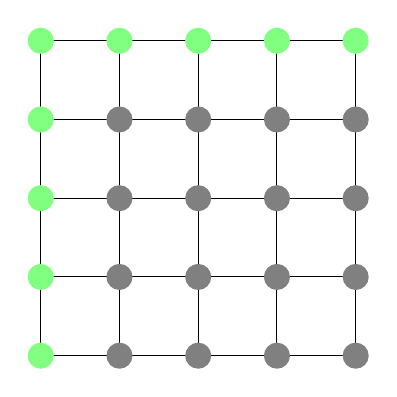
\begin{tikzpicture}[x=1cm,y=1cm]
\def\Factor{1}
\foreach \Column in {1,...,5}
{
  \foreach \Row in {1,...,5}
  {
    \ifnum\Row = 1\relax
      \def\Shape{circle}
      \def\Color{green!50}
      \node[
      minimum size=0.2cm,
      shape=\Shape,
      fill=\Color,
      font=\footnotesize,
      ] 
      (a\Column\Row)
      at (\Factor*\Row,-\Factor*\Column) 
      {};
     \else
     \ifnum\Column = 1\relax
      \def\Shape{circle}
      \def\Color{green!50}
      \node[
      minimum size=0.2cm,
      shape=\Shape,
      fill=\Color,
      font=\footnotesize,
      ] 
      (a\Column\Row)
      at (\Factor*\Row,-\Factor*\Column) 
      {};
\else
      \def\Shape{circle}
      \def\Color{black!50}
    \node[
      minimum size=0.2cm,
      shape=\Shape,
      fill=\Color,
      font=\footnotesize,
      ] 
      (a\Column\Row)
      at (\Factor*\Row,-\Factor*\Column) 
      {};
      \fi
      \fi
  }
}
\begin{pgfonlayer}{background}
\draw (a11) grid[step=\Factor] (a55);
\end{pgfonlayer}
\end{tikzpicture}
$$
We are interested in the quotients we pass through. On the vertical, we pass through $\{1\},\{1\}$, etc., and on the horizontal, we pass through $B_1/B_0, B_2/B_1$, etc. This route gives us the second composition series. Consider, instead, the route below.  
$$
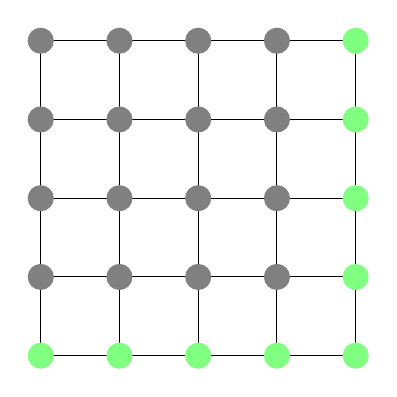
\begin{tikzpicture}[x=1cm,y=1cm]
\def\Factor{1}
\foreach \Column in {1,...,5}
{
  \foreach \Row in {1,...,5}
  {
    \ifnum\Row = 5\relax
      \def\Shape{circle}
      \def\Color{green!50}
      \node[
      minimum size=0.2cm,
      shape=\Shape,
      fill=\Color,
      font=\footnotesize,
      ] 
      (a\Column\Row)
      at (\Factor*\Row,-\Factor*\Column) 
      {};
     \else
     \ifnum\Column = 5\relax
      \def\Shape{circle}
      \def\Color{green!50}
      \node[
      minimum size=0.2cm,
      shape=\Shape,
      fill=\Color,
      font=\footnotesize,
      ] 
      (a\Column\Row)
      at (\Factor*\Row,-\Factor*\Column) 
      {};
\else
      \def\Shape{circle}
      \def\Color{black!50}
    \node[
      minimum size=0.2cm,
      shape=\Shape,
      fill=\Color,
      font=\footnotesize,
      ] 
      (a\Column\Row)
      at (\Factor*\Row,-\Factor*\Column) 
      {};
      \fi
      \fi
  }
}
\begin{pgfonlayer}{background}
\draw (a11) grid[step=\Factor] (a55);
\end{pgfonlayer}
\end{tikzpicture}
$$
Here, we go through $\{1\}, \{1\}$, etc. and $A_1/A_0, A_2/A_1$, etc. This corresponds to the first composition series. 

Now consider the following path.
$$
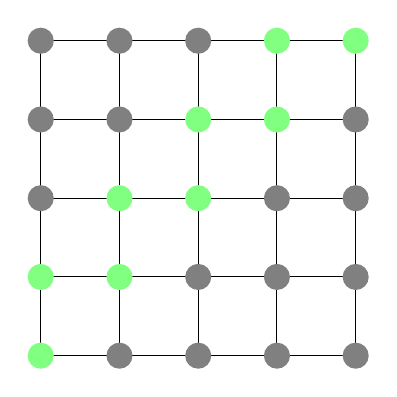
\begin{tikzpicture}[x=1cm,y=1cm]
\def\Factor{1}
\foreach \Column in {1,...,5}
{
  \foreach \Row in {1,...,5}
  {
    \ifnum\Row = \numexpr6 - \Column\relax\relax
      \def\Shape{circle}
      \def\Color{green!50}
      \node[
      minimum size=0.2cm,
      shape=\Shape,
      fill=\Color,
      font=\footnotesize,
      ] 
      (a\Column\Row)
      at (\Factor*\Row,-\Factor*\Column) 
      {};
     \else
     \ifnum\Row = \numexpr5 - \Column\relax\relax
      \def\Shape{circle}
      \def\Color{green!50}
      \node[
      minimum size=0.2cm,
      shape=\Shape,
      fill=\Color,
      font=\footnotesize,
      ] 
      (a\Column\Row)
      at (\Factor*\Row,-\Factor*\Column) 
      {};
\else
      \def\Shape{circle}
      \def\Color{black!50}
    \node[
      minimum size=0.2cm,
      shape=\Shape,
      fill=\Color,
      font=\footnotesize,
      ] 
      (a\Column\Row)
      at (\Factor*\Row,-\Factor*\Column) 
      {};
      \fi
      \fi
  }
}
\begin{pgfonlayer}{background}
\draw (a11) grid[step=\Factor] (a55);
\end{pgfonlayer}
\end{tikzpicture}
$$
Likewise, we will go through other quotients. We want to show that every route has the same quotients up to reordering. We can get from any route to another by repeatedly flipping squares.

Suppose two routes differ by one square. That is, we have 
\begin{center}
\begin{tikzpicture}[node distance=3 cm]
\node (1)  {$A_i\cap B_{j-1}$};
\node (2) [right of = 1]{$A_i \cap B_j$};
\node (3) [below of = 1]{$A_{i-1} \cap B_{j-1}$};
\node (4) [right of = 3]{$A_{i-1}\cap  B_j$};
\draw (1) -- (2);
\draw (2) -- (4);
\draw (1) -- (3);
\draw (3) -- (4);
\end{tikzpicture}
\end{center}
We will just quotient out by $B_{j-1}$ since it is a normal subgroup of everything, so we get 
\begin{center}
\begin{tikzpicture}[node distance=2 cm]
\node (1)  {$A$};
\node (2) [right of = 1]{$X$};
\node (3) [below of = 1]{$\{1\}$};
\node (4) [right of = 3]{$B$};
\draw (1) -- (2);
\draw (2) -- (4);
\draw (1) -- (3);
\draw (3) -- (4);
\end{tikzpicture}
\end{center}
where $X$ is a group and $A$ and $B$ are subgroups of $X$. If $A=B$, then either route gives $A$ and $X/A$ (in the same order), so the factors don't change. Suppose $A\ne B$. We know $A, B$ are simple normal subgroups of $X$, so $X = A\times B$. Now, either route gives $A$ and $B$ (in opposite orders). Therefore, every time we change a route, we either keep the order of factors the same or switch them. 

So any two routes have the same factors up to reordering. 
\end{proof}
This also works for groups with operators (for example, modules over a ring).

Now we have a framework for transforming many problems involving groups into problems involving simple groups. 

How do we classify simple groups? There are $18$ infinite series of them, including $\Ag_n$ for $n\ge 5$ and $\PSL_n(\F_q)$ for $n\ge 2$ or $n\ge 3$ if $q=2,3$. There are also $26$ sporadic groups, and the smallest is $\MM_{11}$ of order $7920$ while the largest is the monster group $\MM$ of order approximately $10^{54}$. This classification is one of the greatest feats of mathematics. The proof kind of works by looking at the centralizers of an involution. (A group has an involution if and only if it has even order, so the proof starts by showing that all noncyclic simple groups have even order.)


\section{Outer automorphisms}
\begin{definition}
An \defn{inner automorphism} of a group $G$ is an automorphism that takes an element $x\in G$ to $gxg\inv$ for some $g\in G$.
\end{definition}
The group of inner automorphisms is $\Inn(G) = G / \ZZ(G)$. The quotient $\Out(G) = \Aut(G)/\Inn(G)$ is called the \defn{outer automorphisms} of $G$, and we get an exact sequence
$$
\{1\} \longrightarrow \ZZ(G) \longrightarrow G\longrightarrow \Aut(G) \longrightarrow \Out(G) \longrightarrow \{1\}.
$$
Since we generally know $G$ and $\ZZ(G)$, determining $\Aut(G)$ depends on determining $\Out(G)$.
\begin{example}
Suppose $G = (\Zmod 2)^2$. Then $\ZZ(G) = G$, so $\Inn(G) = \{1\}$. So $\Out(G) = \Aut(G)$, and we know $\Aut(G) = \Sg_3$.
\end{example}

For most groups, the automorphisms are usually easy to find. Suppose $G = \PSL_n(\F_q)$. Then $\Aut(G)$ consists of inner automorphisms, conjugations by elements of $\GL_n(\F_q)$,  field automorphisms $\F_q\longrightarrow \F_q$, and $g\mapsto \tp{(g\inv)}$. Indeed, $\Aut(G)$ is generated by these obvious automorphisms, and this is usually the case.

Suppose $G= \Ag_n$. Then the obvious automorphisms are $\Sg_n$, and if $n\ne 6$, this gives all automorphisms of $G$, so $\Out(G) = \Zmod 2$. When $n=6$, we find $\Out(\Ag_n) = \Zmod 2 \times \Zmod 2$. (The sporadic group $\MM_{11}$ has subgroup fixing a point of order $720$ and is composed of $\Ag_6$ with an unexpected automorphism of it.)

Let's consider outer automorphisms of $\Sg_6$. Observe that $\Sg_5$ has a subgroup of index $6$ of order $20$, which is a Frobenius group of order $20$. This gives a nontrivial homomorphism $\Sg_5\longrightarrow \Sg_6$ ($\Sg_5$ acts transitively on a set of $6$ elements), so $\Sg_5\subset \Sg_6$ not fixing a point. In fact, $\Sg_6$ has $6+6$ subgroups of $\Sg_5$ (usually $\Sg_n$ has $n$ subgroups $\Sg_{n-1}$). The group $\Sg_6$ has a transitive $\Sg_5$ subgroup of index $6$. This gives a homomorphism $\Sg_6\longrightarrow\Sg_6$ acting on the $6$ cosets of this subgroup. This is not an inner automorphism, so $\Sg_6$ has an outer automorphism. 

We want to write down an outer automorphism explicitly. The group $\Sg_6$ is generated by the $5$ transpositions:
$$
\Sg_6 : \dynkin [Coxeter]A{5}
$$
(So for the transpositions $\tau_1,\hdots, \tau_5$, if $i < j$, then $\tau_i^2 = 1$, $(\tau_i\tau_j)^2=1$ if $j \ne i+1$, and $(\tau_i\tau_j)^3=1$ if $j = i+1$.) We want to find $\sigma_1 ,\hdots,\sigma_5$ with the same relations. Then we can get a homomorphism $\Sg_6\longrightarrow\Sg_6$ by $\tau_i \mapsto \sigma_i$. This automorphism will not be inner since the $\sigma_i$ are not transpositions. So each $\sigma_i$ is of the form $(*\ *)(*\ *)(*\ *)$ (a product of three transpositions), since the product will be of order $3$ or order $2$. Consider $\sigma_1 = (1\ 2)(3\ 4)(5\ 6)$. Then $\sigma_2$ can have no transposition in common with $\sigma_1$, so $\sigma_2 = (2\ 3)(4\ 5)(6\ 1)$. The element $\sigma_3$ must have no transposition in common with $\sigma_2$ and one in common with $\sigma_1$, so $\sigma_3 = (1\ 2)(3\ 5)(4\ 6)$. The element $\sigma_4$ must have one transposition in common with $\sigma_1$ and $\sigma_2$ but none in common with $\sigma_3$, so $\sigma_4 = (3\ 4)(6\ 1)(2\ 5)$. Finally, $\sigma_5$ must have one transposition in common with $\sigma_1,\sigma_2,\sigma_3$ but none in common with $\sigma_4$, so we get $\sigma_5 = (1\ 2)(4\ 5)(6\ 3)$. So we get our explicit outer automorphism of $\Sg_6$:
\begin{align*}
(1\ 2) &\mapsto (1\ 2)(3\ 4)(5\ 6),\\
(2\ 3) &\mapsto (2\ 3)(4\ 5)(6\ 1),\\
(3\ 4) &\mapsto (1\ 2)(3\ 5)(4\ 6),\\
(4\ 5) &\mapsto (3\ 4)(6\ 1)(2\ 5),\\
(5\ 6) &\mapsto (1\ 2)(4\ 5)(6\ 3).
\end{align*}
(Dr. Borcherds provides illustrations at around 16:00 of lecture 30.) 

No other symmetric groups have nontrivial outer automorphism group. Let $G = \Sg_n$. Suppose $\sigma\in \Aut(G)$ takes transpositions to transpositions. Then $\sigma$ is inner. We can reconstruct $n$ points from the transpositions (though $n=3$ takes some more work), by knowing the transpositions, so any $\sigma $ also acts on the $n$ points of $\Sg_n$ and must be an inner automorphism of $\Sg_n$. Are there automorphisms that do not preserve transpositions? The number of transpositions of $\Sg_n $ is $n(n-1)/2$, and the number of products of two transpositions is $n(n-1)(n-2)(n-3)/2^32!$. The number of products of three transpositions is similarly derived.
\begin{center}
\begin{tabular}{cccccccc} 
	%\longrightarrowprule
    {$G$} & {$\#$ transpositions} & {$\#$ products of two transpositions} & {$\#$ products of three transpositions} \\
    \midrule
    {$\Sg_1$} & $0$ & $0$ & $0$ \\ 
    {$\Sg_2$} & $1$ & $0$ & $0$ \\
    {$\Sg_3$} & $3$ & $0$ & $0$ \\
    {$\Sg_4$} & $6$ & $3$ & $0$ \\
    {$\Sg_5$} & $10$ & $15$ & $0$ \\
    {$\Sg_6$} & $15$ & $45$ & $15$ \\
    {$\Sg_7$} & $21$ & $105$ & $105$ \\
    {$\Sg_8$} & $28$ & $210$ & $420$ \\
    %\bottomrule
\end{tabular}
\end{center}
We notice that the number of transpositions is the same as the number of products of three transpositions for $\Sg_6$. If an outer automorphism takes transpositions to some other conjugacy class, these conjugacy classes must have the same order. This happens for $\Sg_6$. Extending this table, we get
\begin{center}
\begin{tabular}{cccccccc} 
	%\longrightarrowprule
    {$G$} & {$\# \{ (*\ *)\}$} & {$\# \{ (*\ *)(*\ *))\}$} & {$\# \{ (*\ *)(*\ *)(*\ *)\}$} & {$\# \{ (*\ *)(*\ *)(*\ *)(*\ *)\}$} \\
    \midrule
    {$\Sg_1$} & $0$ & $0$ & $0$ & $0$\\ 
    {$\Sg_2$} & $1$ & $0$ & $0$& $0$\\ 
    {$\Sg_3$} & $3$ & $0$ & $0$ & $0$\\ 
    {$\Sg_4$} & $6$ & $3$ & $0$ & $0$\\ 
    {$\Sg_5$} & $10$ & $15$ & $0$ & $0$\\ 
    {$\Sg_6$} & $15$ & $45$ & $15$ & $0$\\ 
    {$\Sg_7$} & $21$ & $105$ & $105$ & $0$\\ 
    {$\Sg_8$} & $28$ & $210$ & $420$ & $105$\\ 
    %\bottomrule
\end{tabular}
\end{center}
There are no outer automorphisms for any other $\Sg_n$, since the numbers in the last (three) columns are greater than $n(n-1)/2$ for $n>6$. This computation is straightforward. 

\section{Free groups}
\begin{definition}
The \defn{free abelian group} $G$ on commutative elements $\alpha_1,\hdots,\alpha_n$ is the universal abelian group generated by the $\alpha_i$ (with basis $\{\alpha_i\}$). That is, $G = \bigoplus_n \Z$.
\end{definition}

(Universal property.) If $F$ is a free abelian group and $A$ is an abelian group then there is a unique homomorphism from $F$ to $A$. In particular, $\rank F$ (the number of generators) is well-defined. We can see this by observing that there are $2^n$ homomorphisms from the free group on $n$ generators to $\Zmod 2$.

Let $\Z^n$ be a free abelian group. All of its subgroups are free abelian of rank $\le n$. We can choose a basis $\{a_1,\hdots,a_n\}$ so that the subgroup is of the form $\ang{r_1a_1,\hdots, r_na_n}$ where the $r_i$ are nonnegative integers.

\begin{proof}
See the classification of finitely generated abelian groups.
\end{proof}

A free abelian group corresponds to a lattice.

We want to consider the nonabelian analogues to free abelian groups, but first, we should consider ``free monoids'' (monoids are groups without inverses). The obvious way to construct a free monoid on elements 
$\alpha,\beta,\gamma,\hdots$ is to take all words on $\alpha,\beta,\gamma,\hdots$. If $F(\alpha,\beta)$ is a free monoid and $M$ is a monoid, then if we choose two elements in $M$, then there is a unique homomorphism from $F(\alpha,\beta)$ to $M$ where $\alpha$ maps to the first element and $\beta$ to the second.

Suppose $M$ is a monoid. We form the smallest equivalence relation $\sim$ on $M$ such that if $x\sim a$ and $y\sim b$ then $xy \sim ab$ and $yx \sim ba$ for all $x,y,a,b\in M$.

Now we form a free group by taking a free monoid on $\alpha, \alpha\inv,\beta,\beta\inv,\hdots$ and modding out by $\sim$ such that $\alpha\alpha\inv \sim \alpha\inv\alpha \sim 1$, etc. If $G$ is a group with elements $\alpha,\beta,\gamma$, we have a unique homomorphism $F(a,b,c) \longrightarrow G$ defined by $a\mapsto \alpha$, $b\mapsto \beta$, $c\mapsto \gamma$, etc. for more generators. (This is the universal property.) Again, the rank is well-defined in the same way (the free group on $2$ generators is distinct from the free group on $3$ generators, for example).

Let's try to write down the elements of a free group. In the free monoid, we might have elements like $1,\alpha,\beta,\alpha\inv,\beta\inv,\alpha^2,\alpha\beta,\alpha\beta\inv, \alpha\alpha\inv$, etc. In the free monoid, the element $\alpha\alpha\inv$ is distinct from $1$, but in the free group, $\alpha\alpha\inv =1$. Another element like $\alpha\alpha\beta\beta\inv \alpha\inv\beta\alpha\inv$ is just $\alpha\beta\alpha\inv$ in the free group. Every word is equivalent to a reduced word (that does not contain $xx\inv$ or $x\inv x$). 

\begin{proposition}
If $2$ reduced words are distinct they are distinct in the free group. That is, if a reduced word is nonempty, then it is nontrivial in the free group.
\end{proposition}
\begin{proof}
This reduces to showing that, given a reduced word in $\alpha,\alpha\inv,\beta,\beta\inv,\hdots$ one can always find a group $G$ with elements $a,a\inv,b,b\inv,\hdots$ such that this word is not $1$. If the word has length $n$, take $G=\Sg_{n+1}$.
\end{proof}
\begin{example} %16:30 (https://www.youtube.com/watch?v=-uFamgRrCl0&list=PL8yHsr3EFj51pjBvvCPipgAT3SYpIiIsJ&index=31)
Take the reduced word $\alpha^2\beta\alpha\inv\beta\alpha\beta\alpha^2\beta^{-3}$. Can you find a group with elements $a,b$ such that this reduced word is not equal to $1$? This is a word of length $12$, so we take $13$ points and and draw arrows such that $\alpha,\beta$ correspond to a right-pointing arrow between points, and $\alpha\inv$, $\beta\inv$ correspond to a left-pointing arrow. We now have a partial permutation on $13$ points, and since no triplet of points has $\alpha\alpha\inv$ or $\beta\beta\inv$ (the word is reduced), we can complete the permutation. Hence we see that this reduced word is not the identity in $\Sg_{13}$.
\end{example}

\begin{definition}
A group $G$ is \defn{residually finite} if for any nonidentity element $g\in G$ we can define a homomorphism from $G$ to a finite group $H$ such that $g$ has nonidentity image.
\end{definition}

We have actually proven that free groups are residually finite. 
\begin{example}
The groups $(\Q,+)$ and $(\R,+)$ are not residually finite (neither is any infinite simple group).
\end{example}

Why not define the free group as the set of reduced words? Well,  proving associativity is a nightmare. 

The free group on two generators impossible to draw in Euclidean space, so we need to draw it in hyperbolic space. See figure 5. In some sense, free abelian groups live in Euclidean space whereas free groups live in hyperbolic space.
\begin{figure}
\centering
\includegraphics[scale=0.3]{images/free_group_on_two_generators}
\caption{The Cayley graph of the free group on two generators embedded in the Poincar\'e disk model.}
\end{figure}

We know that any subgroup of a free abelian group is free abelian of rank less than or equal to the free abelian group. Any subgroup of a free group is free, but the rank can increase. (The abelian group on $3$ generators is a subgroup of the free group on $2$ generators, for example.)

\section{Subgroups of free groups}
\begin{proposition}
Subgroups of free groups are free.
\end{proposition}

An index $n$ subgroup of any group $G$ is a transitive action of $G$ on $n$ points (where one is marked). Transitive actions of a free group on $n$ points are easy to imagine. If we draw $n$ points, draw arrows between these points corresponding to actions of the generators, and mark one point, we get an index $n$ subgroup defined by all paths from the marked point to itself up to homotopy. This subgroup, therefore, is the fundamental group of the previously described path with respect to the base point.

What is the fundamental group of a graph? Consider the graph below, where the black node is the base point.
\begin{center}
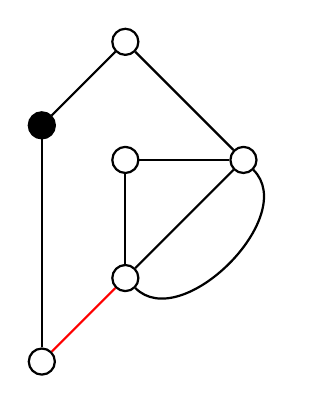
\begin{tikzpicture}
	[node distance={15mm}, 
	thick, 
	main/.style = {draw, circle,minimum size=4pt},
	marked/.style = {draw, circle, fill = black,minimum size=4pt}] 
\node[main] (1) {}; 
\node[marked] (2) [below left of=1] {}; 
\node[main] (3) [below of = 1] {}; 
\node[main] (4) [right of=3] {}; 
\node[main] (5) [below of=3] {}; 
\node[main] (6) [below left of=5] {}; 
\draw (1) -- (4); 
\draw (1) -- (2); 
%\draw (1) to [out=135,in=90,looseness=1.5] (5); 
%\draw (1) to [out=180,in=270,looseness=5] (1); 
\draw (3) -- (4); 
\draw (5) -- (4); 
\draw[red] (5) -- (6);
\draw (2) -- (6);
\draw (3) -- (5);
\draw (5) to [out=315, in=315, looseness=1] (4); 
%\draw[->] (5) to [out=315, in=315, looseness=2.5] (3); 
%\draw[->] (6) -- node[midway, above right, sloped, pos=1] {+1} (4); 
\end{tikzpicture} 
\end{center}
We can simplify this graph without changing the fundamental group. We can take the red edge and contract it to a point:
\begin{center}
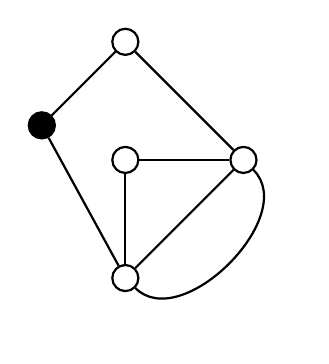
\begin{tikzpicture}
	[node distance={15mm}, 
	thick, 
	main/.style = {draw, circle,minimum size=4pt},
	marked/.style = {draw, circle, fill = black, minimum size=4pt}] 
\node[main] (1) {}; 
\node[marked] (2) [below left of=1] {}; 
\node[main] (3) [below of = 1] {}; 
\node[main] (4) [right of=3] {}; 
\node[main] (5) [below of=3] {}; 
\draw (1) -- (4); 
\draw (1) -- (2); 
%\draw (1) to [out=135,in=90,looseness=1.5] (5); 
%\draw (1) to [out=180,in=270,looseness=5] (1); 
\draw (3) -- (4); 
\draw (5) -- (4); 
\draw (2) -- (5);
\draw (3) -- (5);
\draw (5) to [out=315, in=315, looseness=1] (4); 
%\draw[->] (6) -- node[midway, above right, sloped, pos=1] {+1} (4); 
\end{tikzpicture} 
\end{center}

``Any loop in the first graph corresponds to a loop in the second graph,'' so the fundamental group is the same. If we continue to contract edges, we wind up with one vertex with five distinct edges from it to itself. The fundamental group of that graph is clearly the free group on five generators (since we have five loops). So the fundamental group is a free group on the ``loops.'' So any subgroup of a free group is free. \hfill \qed

How do we write down the set of generators for this free group? 
\begin{example}
Consider the free group on $2$ generators and the action of it on two points. If we fix a point, each generator either fixes the points or swaps them, and both generators cannot fix a point since the graph is connected, so we get three possible ways to make the two points into a connected graph with two generators. Suppose $a$ (red) and $b$ (blue) are the generators:
\begin{center}
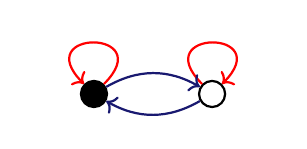
\begin{tikzpicture}
	[node distance={15mm}, 
	thick, 
	main/.style = {draw, circle,minimum size=1pt},
	marked/.style = {draw, circle, fill = black, minimum size=1pt}] 
\node[marked] (1) {};
\node[main] (2) [right of =1]{};
\draw[->, red] (1) to [looseness=10, out= 45, in=135,] (1);
\draw[->, red] (2) to [looseness=10, out= 135, in=45,] (2);
\draw[->, MidnightBlue] (1) to [bend left,] (2);
\draw[->, MidnightBlue] (2) to [bend left,] (1);
\end{tikzpicture}
\end{center}
We contract this graph by annihilating the bottom blue line, and then we get a point with three distinct loops (three generators). The first $a$-loop remains $a$. The second $a$-loop is not $a$: it actually corresponds to going from the marked point to the unmarked point, then around the second $a$-loop, so we get $b ab\inv$. The remaining loop corresponds to $b^2$, not $b$, since we have to go from the marked point to the unmarked point back to the marked point. So the subgroup of index $2$ is a free group on $3$ generators ($a$, $bab\inv$, $b^2$). That is, the free group on three generators is a subgroup of the free group on two generators.
\end{example}

Suppose $G$ is index $k$ in $F_n$ (the free group on $n$ generators). How many generators does $G$ have? We draw the graph for $G$ with $k$ points and $nk$ edges. The Euler characteristic of the graph is $\chi= k-kn$, so $\chi$ does not change when we contract an edge of the graph. So the graph with one point has characteristic $\chi = k-nk$, which is $1-\textrm{the number of loops}$. So the number of loops is $1 + nk - k$, and the number of loops is the number of generators.

Suppose we have a map $F_2\twoheadrightarrow \Sg_3$. (Recall that $\Sg_3$ has two generators $a$ and $b$ satisfying $a^2=1$, $b^2=1$, and $(ab)^3 = 1$.) Suppose we want to find the generators for the kernel of this map. ``Well that sounds like a completely daft question: I just told you the relations that give you $\Sg_3$ are these three elements, so surely the kernel is just the free group on these three elements: $a^2$, $b^2$, and $(ab)^3$. Well, no: that's wrong.'' These three elements do not generate the kernel, but these elements together with their conjugates do (the kernel must be normal, and these elements do not generate a normal subgroup). The subgroup is index $6$, so the kernel should be a free group on $7$ generators. 

To find these generators, we write down an action of $F_2$ on $6$ points:
\begin{center}
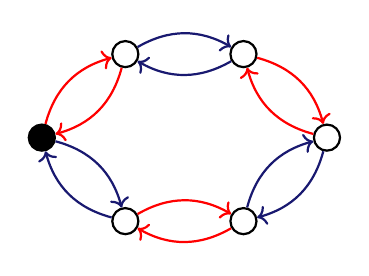
\begin{tikzpicture}
	[node distance={15mm}, 
	thick, 
	main/.style = {draw, circle,minimum size=4pt},
	marked/.style = {draw, circle, fill = black, minimum size=4pt}] 
\node[main] (1) {};
\node[main] (2) [right of =1]{};
\node[marked] (3) [below left of = 1] {};
\node[main] (4) [below right of = 2] {};
\node[main] (5) [below right of = 3] {};
\node[main](6) [below left of = 4] {};
\draw[->, red] (1) to [bend left,] (3);
\draw[->, red] (3) to [bend left,] (1);
\draw[->, MidnightBlue] (3) to [bend left,] (5);
\draw[->, MidnightBlue] (5) to [bend left,] (3);
\draw[->, red] (5) to [bend left,] (6);
\draw[->, red] (6) to [bend left,] (5);
\draw[->, MidnightBlue] (1) to [bend left,] (2);
\draw[->, MidnightBlue] (2) to [bend left,] (1);
\draw[->, red] (2) to [bend left,] (4);
\draw[->, red] (4) to [bend left,] (2);
\draw[->, MidnightBlue] (4) to [bend left,] (6);
\draw[->, MidnightBlue] (6) to [bend left,] (4);
\end{tikzpicture}
\end{center}
This particular graph looks very symmetric. In particular, there is a symmetry taking any vertex to any other vertex, corresponding to the fact that the subgroup is normal. The conjugate of the fundamental group of the marked point by some element of the free group will be the fundamental group of another point. The fundamental group of each point is the same, so there is a symmetry taking a point to another.  Now we contract some edges to get seven arrows, and each will correspond to a generator:
\begin{center}
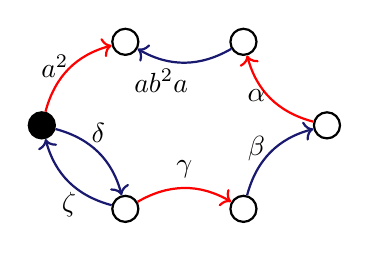
\begin{tikzpicture}
	[node distance={15mm}, 
	thick, 
	main/.style = {draw, circle,minimum size=4pt},
	marked/.style = {draw, circle, fill = black, minimum size=4pt}] 
\node[main] (1) {};
\node[main] (2) [right of =1]{};
\node[marked] (3) [below left of = 1] {};
\node[main] (4) [below right of = 2] {};
\node[main] (5) [below right of = 3] {};
\node[main](6) [below left of = 4] {};
\draw[->, red] (3) to [bend left,above, align=left] node [near start] {\color {black}$a^2$} (1);
\draw[->, MidnightBlue] (3) to [bend left, above, align=left] node [midway] {\color {black}$\delta$} (5);
\draw[->, MidnightBlue] (5) to [bend left, below, align=left] node [midway] {\color {black}$\zeta$} (3);
\draw[->, red] (5) to [bend left, above, align=right] node [midway] {\color {black}$\gamma$} (6);
\draw[->, MidnightBlue] (2) to  [bend left, below, align=left] node [near end] {\color {black}$a\inv b^2a$} (1);
\draw[->, red] (4) to [bend left, below, align=right] node [near end] {\color {black} $\alpha $} (2);
\draw[->, MidnightBlue] (6) to [bend left, above, align=left] node [near start] {\color {black}$\beta$} (4);
\end{tikzpicture}
\end{center}
where 
\begin{align*}
\alpha &= a\inv b\inv a^2ba, \\
\beta &= a\inv b\inv a\inv b^2aba,\\
\gamma &= a\inv b\inv a\inv b\inv a^2baba\\
\delta &= a\inv b\inv a\inv b\inv a\inv b, \textrm{ and} \\
\zeta &= bababa.
\end{align*}
So the set of seven generators is $\{a^2,\, a\inv b^2a, \,\alpha,\,\beta,\,\gamma,\,\delta,\,\zeta\}$.

\end{document}
